\documentclass{article}
\usepackage[a4paper, total={6in, 8in}]{geometry}
\usepackage[utf8]{inputenc}
\usepackage[affil-it]{authblk}
\usepackage[english]{babel}
\usepackage{polski}

% packages for title page
\usepackage{siunitx}
\usepackage[export]{adjustbox}
\usepackage{graphicx, wrapfig}
\usepackage{tabularx}

\usepackage{amsfonts}
\usepackage{amssymb}
\usepackage{amsmath}
\usepackage{mathrsfs}

\usepackage{xcolor}
\usepackage{subfigure}
\usepackage[super]{nth}
\usepackage{indentfirst}
\usepackage{algorithm,algorithmic}
\usepackage{enumerate}
\usepackage[toc,page]{appendix}

\usepackage{amsthm}
\usepackage{pdfcomment}
\usepackage{textgreek}

\usepackage[siunitx,americaninductors]{circuitikz}
\usepackage{schemabloc}
\usetikzlibrary{circuits}
\usepackage{tikz, pgfplots}
\usetikzlibrary{shapes,arrows}
\usepackage{verbatim}

\begin{document}

\clearpage\thispagestyle{empty}
\begin{tabular}{m{2.15cm} m{8.0cm} m{3.2cm}}
        \includegraphics[width=2.15cm]{title_pages/school_logos/pl_logo2.jpg} 
        &
        \begin{tabular}{c}
            \LARGE
             Lodz University of Technology\vspace{0.25cm}\\
             
             \Large
             Faculty of Mechanical Engineering\vspace{0.25cm}\\
             \Large
             Institute of Turbomachinery
        \end{tabular}
        & 
        \includegraphics[width=3.2cm]{title_pages/school_logos/PL_logo1.png}
\end{tabular}

\vspace{1.0cm}
\begin{flushleft}
\LARGE
inż. Michał Wilczek
\\
\Large
Index no: 220242
\end{flushleft}

\begin{center}
    \vspace*{1cm}
    \LARGE
    \text{Master thesis}
    \Large
    \text{in}
    
    \text{Advanced Mechanical Engineering}
    \vspace{2.0cm}
   
   \LARGE
    \textbf{Heat Propagation Modelling in Superconducting Magnets based on Quench Velocity}
    \vspace{1.5cm}

    \text{Lodz University of Technology Supervisor}
    
    \text{dr hab. inż. Artur Gutkowski}
    \vspace{1.0cm}
   
    \text{CERN Supervisor}
    
    \text{Michał Maciejewski, PhD}
    \vspace{1.0cm}
            
    \text{Łódź, February 2020}
\end{center}
\newpage

\clearpage\thispagestyle{empty}
\tableofcontents
\clearpage\thispagestyle{empty}

\section*{Notation}

\begin{table}[h!]
    \vspace{-1.em} 
    \fontsize{10}{10}
    \selectfont 
    \renewcommand{\arraystretch}{1.5}
    \begin{center}
    \begin{tabular}{ l l }  
    \hline
    $A_\text{Cu}$ & cross-sectional area of copper in a wire \\  
    $B_\text{c20}$ & intercepts of critical surface along magnetic field axis \\  
    $C_\text{p, equiv}$ & equivalent specific heat capacity of a wire \\  
    $C_\text{p, Cu}$ & specific heat capacity of copper \\   
    $C_\text{p, NbTi}$ & specific heat capacity of NbTi \\  
    $d_\text{strand}$ & real diameter of a wire \\  
    $d_\text{strand, red}$ & reduced diameter of a wire \\   
    $f_\text{Cu}$ &  copper volumetric ratio in a wire\\        
    $f_\text{NbTi}$ &  NbTi volumetric ratio in a wire\\   
    $T_\text{c}$ & critical temperature \\
    $T_\text{c0}$ & intercepts of critical surface along temperature axis \\
    $RRR$ & residual resistivity ratio \\
    \hline
     \end{tabular} 
    \end{center}  
 \end{table}
\newpage

% official introduction of the Master thesis
\section{Introduction}

\subsection{About CERN}

\subsection{Superconductors}

\begin{figure}[ht!]
\centering
\includegraphics[width=0.49\linewidth]{figures/introduction/critical_surface_scheme.png}
\caption{Schematic of the critical surface of $\text{Nb}_\text{3}\text{Sn}$ and Nb-Ti \cite{evans_marvel_of_technology}}
\label{fig:scheme_critical_surface}
\end{figure}



\subsection{Quench Problem}

    \subsubsection{Copper Resistivity}
    Copper residual resistivity ratio according to NIST: 
    \begin{equation}
    RRR = \frac{\rho(T=273~\text{K}, B=0~\text{T})}{\rho(T=4~\text{K}, B=0~\text{T})}
    \end{equation}
    
    \subsubsection{Critical Parameters for Superconductivity}
    Critical current:
    \begin{equation}
        I_\text{c}(T) = I \frac{T-T_\text{cs}}{T_\text{c}-T_\text{cs}}
    \end{equation}
    \\
    Critical temperature:
    \begin{equation}
        T_\text{c}(B) = 9.2 \cdot [1- \frac{B}{14.5}]^{0.59}~\text{for}~B~<~10~\text{T}
    \end{equation}
    \\
    Critical magnetic field: 
    \begin{equation}
        B_\text{c2}(T) = B_\text{c2}(T=0) \cdot [1-(\frac{T}{T_\text{c}(B=0)})^{n}],
    \end{equation}
    where
    $B_\text{c2}(T=0)=14.5~\text{T}$, $T_\text{c}(B=0)=9.2~\text{K}$, $n=1.7$.

    \subsubsection{Current Flow in Copper Matrix}
    
    Current sharing temperature: 
    \begin{equation}
        T_\text{cs} = T_\text{c} (1 - \frac{I}{\text{c}_1 + \text{c}_2 B }),
    \end{equation}
    where $\text{c}_1=3449~\text{A}$ and $\text{c}_2=-257~\text{AT}^{-1}$
    \\
    Current in copper matrix: 
    \begin{equation}
        \left\{ \begin{array}{lll}
        I_\text{Cu} = 0 & \text{for}~T < T_\text{cs} \\ \\
        I_\text{Cu} = I - I_\text{c} & \text{for}~T_\text{cs} \leq T<T_\text{c}  \\ \\
        I_\text{Cu} = I & \text{for}~T_\text{cs} \leq T
        \end{array} \right.
    \end{equation}
    \\
    Joule heating: 
    \begin{equation}
        \left\{ \begin{array}{lll}
        q_\text{Joule} = 0 & \text{for}~T < T_\text{cs} \\ \\
        q_\text{Joule} = \rho_\text{Cu}(T, B) \frac{(I-I_\text{c})^2}{{\text{a}_\text{Cu}}^2}& \text{for}~T_\text{cs} \leq T<T_\text{c}  \\ \\
        q_\text{Joule} = \rho_\text{Cu}(T, B) \frac{I^2}{{\text{a}_\text{Cu}}^2} & \text{for}~T_\text{cs} \leq T
        \end{array} \right.
    \end{equation}

    \begin{figure}[ht!]
    \centering
    \includegraphics[width=0.49\linewidth]{figures/skew_quad_bcs/magnetic_field_mapping/Heat_Generation_Curve_B_3.png}
    \caption{Heat Generation Curve as a function of temperature for B=3 T}
    \label{fig:H_gen_curve}
    \end{figure}
    
\subsection{Accelerator Magnets}
What type of magnets can we find? \\
How are they protected? \\
Passive and active protections \\ 
Self-protectability

\subsection{Analyses in Superconductors}

\subsection{Numerical Analyses}

Heat conduction equation: 
\begin{equation}
    \frac{\partial}{\partial x}[k(B) \frac{\partial T}{\partial x}] + q_v = \rho c_p \frac{\partial T}{\partial t}
\end{equation}



\subsection{Thermal Numerical Analyses}

To write in introduction: 
Wilson: \\
- point disturbances (page 74) \\
- minimum propagating zone (MPZ) (same page - up to 80 something...)

% AIM THESIS
\clearpage
\section{Aim of Thesis}
\input{sections/aim_thesis/aim_thesis.tex}

% 1D QUENCH PROPAGATION MODELLING 
\clearpage
\section{1D Quench Propagation Modelling}
\label{section: 1d_quench_propagation_modelling}

In this section, 1D analysis of a single strand is conducted in ANSYS and COMSOL software. There are two cases considered: 

\begin{itemize}
    \item 1D strand analysis without insulation layer,
    \item 1D strand analysis with an external insulation layer.
\end{itemize}

For both cases, the mesh density study is conducted, too. In the given analyses, there are several assumptions made: 

\begin{itemize}
    \item There is no helium cooling.
    \item Temperature in the winding's cross-sectional area is uniform.
    \item When the insulation layer is considered, the longitudinal heat transfer inside the insulation is negligible with respect to the transversal one.
\end{itemize}

The \nth{2} assumption allows one to consider this problem as a 1D longitudinal heat propagation. When the insulation layer is also simulated within the \nth{3} assumption, the analysis becomes a 1D+1D heat propagation problem. It will be further explained in the section \ref{subsection: 1D_quench_propagation_with_insulation}.

\subsection{Geometry}
\label{subsection: 1d_quench_propagation_geometry}

In this thesis, all the simulations are based on the geometry of a skew quadrupole which belongs to the group of high-order corrector magnets designed for the High-Luminosity LHC. The skew quadrupole is developed by LASA laboratories of INFN-Milano. Its geometry is presented in Fig. \ref{fig:Skew_quad_geometry}. Each of the coils of the skew quadrupole (marked in red in the right picture) is positioned in two mechanical supports (marked in grey). The entire magnet is surrounded by an iron yoke (marked in blue). 

\begin{figure}[H]
    \centering
    \includegraphics[width=0.225\linewidth]{sections/1D_quench_modelling/figures/geometry/SkewQuad3D.png}
    \includegraphics[width=0.30\linewidth]{sections/1D_quench_modelling/figures/geometry/Quadrupole_Cross_Section.png}
    \caption{Left: one coil of the skew quadrupole 3D geometry~\cite{marco_prioli_mails}; right: cross-section of the skew quadrupole~\cite[p.~103-105]{hl_lhc_tech_design_report_v01}.}
    \label{fig:Skew_quad_geometry}
\end{figure}

Each coil of the magnet consists of 754 windings. The entire length of one coil equals 841~m. The 1D geometry is based on geometrical parameters of a single strand of a skew quadrupole whose simulations are further described in the next section. As presented in Fig. \ref{fig: 1d_strand_geometry}, the coil consists of a strand with a circular cross-section (in yellow). The composite strand is made of Nb-Ti with copper as a stabiliser. The composite is fully insulated with an S2-glass material (in red). Then, the strand with the insulation layer is immersed in D10 epoxy resin (in blue)~\cite[p.~103-105]{hl_lhc_tech_design_report_v01}.

\begin{figure}[H]
    \centering
    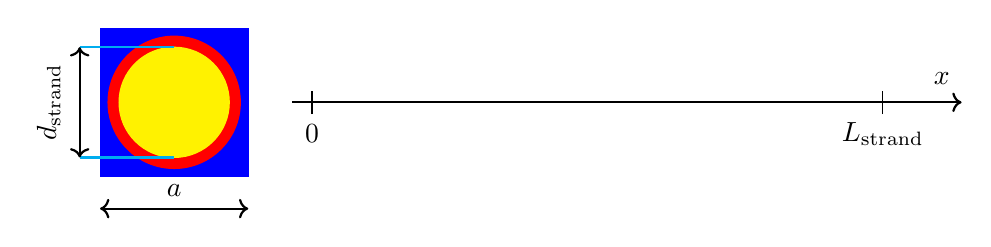
\begin{tikzpicture}[scale = 1]
        \filldraw[blue] (-0.941,-0.941) rectangle (0.941,0.941);
        \filldraw[red] (0,0) circle (0.7+0.07*2);
        \filldraw[yellow] (0,0) circle (0.7);
        \draw[thick, cyan] (-0.8*1.5,0.7) -- (0,0.7);
        \draw[thick, cyan] (-0.8*1.5,-0.7) -- (0,-0.7);
        \draw[black, thick, <->] (-0.75*1.6,0.7) -- (-0.75*1.6,-0.7);
        \node[scale = 1, rotate=90] at (-1.1*1.45, 0) {$d_\text{strand}$};
        \draw[thick,<->] (-0.941,-0.9*1.5) -- (0.941,-0.9*1.5);
        \node[scale = 1] at (0, -0.7*1.6) {$a$};
        \draw[thick,->] (1.5,0) -- (10.0,0);
        \draw[thin] (1.75,-0.15) -- (1.75,0.15);
        \draw[thin] (9,-0.15) -- (9,0.15);
        
        \node[scale = 1] at (9.75, 0.3) {$x$};
        \node[scale = 1] at (9, -0.4) {$L_\text{strand}$};
        \node[scale = 1] at (1.75, -0.4) {0};
        
    \end{tikzpicture}
    \caption{1D strand geometry.}
    \label{fig: 1d_strand_geometry}
\end{figure}

The parameters of the skew quadrupole are presented in Table \ref{table:skew_quad_params_table_basic}. None of the presented parameters change in the remainder of the thesis. The last two: $(i)$ residual resistivity ratio, RRR, $(ii)$ copper-to-superconductor ratio, $r_\text{Cu/Nb-Ti}$ are obtained from the measurements of the prototype magnet performed at INFN~\cite{marco_prioli_mails}.

\begin{table}[H]
    \caption{Geometrical parameters of the skew quadrupole \cite{marco_prioli_mails, hl_lhc_tech_design_report_v01}.} 
    \vspace{-1.em} 
    \fontsize{10}{10}
    \selectfont 
    \renewcommand{\arraystretch}{1.5}
    \begin{center}
    \begin{tabular}{ ccc }  
    \hline
    parameter & value & unit \\
    \hline
    strand diameter, $d_\text{strand}$ & 0.7 & [mm] \\
    strand side, $a$ & 0.941 & [mm] \\
    $r_\text{Cu/Nb-Ti}$ & 2.2 & [-] \\
    RRR & 193 & [-] \\  
    \hline 
    \end{tabular}
    \end{center}  
     \label{table:skew_quad_params_table_basic} 
 \end{table}


\subsection{1D Analysis without Insulation}
\label{subsection: 1D_quench_propagation_no_insulation}

\subsection{Geometry, Material Properties and Mesh}

The strand is a composite with a specified non-superconductor to superconductor ratio given as 

\begin{equation}
    \left\{ \begin{array}{ll}
    r_\text{Cu/Nb-Ti} = \frac{f_\text{Cu}}{f_\text{Nb-Ti}} = \frac{A_\text{Cu}}{A_\text{Nb-Ti}}\\ \\
    f_\text{Cu} + f_\text{Nb-Ti} = 1,
    \end{array} \right.
    \label{eqn: non_super_to_super_ratio}
\end{equation}
where $f_\text{Cu}$ -- volumetric fraction of copper, $f_\text{Nb-Ti}$ -- volumetric fraction of Nb-Ti, $A_\text{Cu}$ -- cross-sectional area of copper, $A_\text{Nb-Ti}$ -- cross-sectional area of Nb-Ti. Since both materials are characterised by a~different volumetric heat capacity, the total volumetric heat capacity of a strand given by

\begin{equation}
    C_\text{v, strand} = f_\text{Cu} ~ C_\text{v, Cu} + f_\text{Nb-Ti} ~ C_\text{v, Nb-Ti},
    \label{eqn: cv_equiv}
\end{equation}
where $C_\text{v, Cu}$ -- volumetric heat capacity of copper, $C_\text{v, Nb-Ti}$ -- volumetric heat capacity of Nb-Ti is shown in Fig. \ref{fig:eq_wind_cp}.

\begin{figure}[H]
\centering
    \begin{tikzpicture}
        \begin{axis}[
          no markers,
          width=0.7\linewidth, 
          height = 4.5cm,
          xlabel={$T,~\text{K}$},
          ylabel={$C_\text{v, strand},~\frac{\text{J}}{\text{m}^3 \cdot \text{K}}$},
          xmin=0.0,
          ymin=0.0,
          xmax=300.0
          ]
          \addplot table[x=temperature,y=cv_equiv,col sep=comma] {sections/1D_quench_modelling/figures/other/cv_equivalent.csv}; 
        \end{axis}
    \end{tikzpicture}
    \caption{Strand volumetric heat capacity as a function of temperature for $B=2~\text{T}$ and $r_\text{Cu/Nb-Ti}=2.2$.}
    \label{fig:eq_wind_cp}
\end{figure}

According to the polynomial interpolation fit used in~\cite[p.~46]{material_props_for_heat_transfer_modelling_in_nb3sn_magnets}, thermal conductivity of Nb-Ti increases linearly in the temperature range of $T \in (20, 200)~\text{K}$ and its value changes from 1 to 9~$\frac{\text{W}}{\text{m K}}$. At temperatures below 20~K, the thermal conductivity of Nb-Ti is lower than~$1~\frac{\text{W}}{\text{m K}}$. By comparing the thermal conductivity of Nb-Ti and copper (see in Appendix~\ref{appendix_material_properties_description}), one can assume that the thermal conductivity of Nb-Ti is negligible and only the part of copper contributes to the longitudinal heat propagation, as 
\begin{equation}
    k_\text{strand} = f_\text{Cu} ~ k_\text{Cu} + f_\text{Nb-Ti} ~ k_\text{Nb-Ti} \approx  f_\text{Cu} ~ k_\text{Cu},
    \label{eqn: k_equiv}
\end{equation}
where $k_\text{strand}$ -- thermal conductivity of a strand, $k_\text{Cu}$ -- thermal conductivity of copper, $k_\text{Nb-Ti}$ -- thermal conductivity of Nb-Ti. It is important to highlight that only in Chapter~\ref{chapter: 1d_quench_propagation_modelling}, the thermal conductivity of copper is calculated according to the Wiedemann-Franz formula, as
\begin{equation}
    k_\text{Cu} = 2.45 \cdot 10^{-8} ~ \frac{T}{\rho_\text{Cu}},
    \label{eqn: k_cu_wiedemann_franz}
\end{equation}
where $T$ -- local strand temperature. Wiedeman-Franz formula is used for the sake of comparison of the results with COMSOL in which only such a material property was available. In the remainder of the thesis, the thermal conductivity of copper and all other material properties are calculated according to fits provided by NIST, as described in Appendix~\ref{appendix_material_properties_description}. 

In ANSYS, the element LINK33 was used to solve the task of 1D thermal quench propagation. It is a uniaxial linear element with the ability to conduct heat between its nodes suitable for steady-state and transient analyses~\cite{ansys_element_manual}. Unlike ANSYS, COMSOL does not use explicit element types to define physical equations in a domain. Instead, one has to choose from a list of available physics modules, in this case thermal physics. Therefore, the algebraic physical equations related to heat conduction in COMSOL were applied externally to the nodes belonging to the composite strand. In both tools, a uniformly distributed mesh was used with mesh size equal to 0.1 mm.

\subsection{Initial and Boundary Conditions}

In the superconducting state, the current flows entirely through a superconductor characterised by zero-resistivity. When a quench occurs, the current starts commuting and strand components can be represented as a parallel connection of two resistors, $R_\text{Nb-Ti}$ and $R_\text{Cu}$. Above the critical temperature, the superconductor resistance is much larger than the one of copper, i.e. $R_\text{Nb-Ti} \gg R_\text{Cu}$. Therefore, it is assumed that the current only flows through a copper stabiliser and only this part of the strand contributes to the Joule heating. Over the entire domain of a strand, a heat source is applied as a power density as
\begin{equation}
    q_\text{Joule} = J_\text{strand}^2~\rho_\text{strand} = J_\text{Cu}^2~\rho_\text{Cu}~f_\text{Cu} = \frac{I_\text{Cu}^2}{f_\text{Cu}^2~A_\text{strand}^2}~\rho_\text{Cu}~f_\text{Cu} = \frac{I_\text{Cu}^2}{A_\text{strand}^2}~\frac{\rho_\text{Cu}}{f_\text{Cu}}, 
    \label{eqn: p_dens_equiv}
\end{equation}
where $J_{strand}$ -- current density in a strand, $\rho_\text{strand}$ -- resistivity of a strand, $J_\text{Cu}$ -- current density in copper, $\rho_\text{Cu}$ -- resistivity of copper, $I_\text{Cu}$ -- current in copper stabiliser, $A_\text{strand}$ -- cross-sectional area of a strand. One should notice that the copper resistivity $\rho_\text{Cu}$ should be divided by the non-superconductor fraction as 
\begin{equation}
    \rho_\text{strand} = \frac{\rho_\text{Cu}}{f_\text{Cu}}.
    \label{eqn:strand_resistivity}
\end{equation}

The Gaussian profile of initial temperature is assumed according to 
\begin{equation}
    T(x) = T_\text{init} + (T_\text{max} - T_\text{init}) ~ e^{-(\frac{x}{\alpha})^2},
    \label{eqn: gaussian_temp_ic}
\end{equation}
where $T(x)$ -- temperature profile along x-axis, $T_\text{init}$ -- initial bath temperature of a strand, $T_\text{max}$ -- maximum temperature of in Gaussian profile, $\alpha$ -- shape parameter of Gaussian profile. The initial input parameters for the 1D analysis are depicted in Table~\ref{table: 1d_quench_propagation_analysis_init_temp_input_parameters}. 

\begin{table}[H]
    \caption{Initial temperature input parameters.} 
    \vspace{-1.em} 
    \fontsize{10}{10}
    \selectfont 
    \renewcommand{\arraystretch}{1.5}
    \begin{center}
        \begin{tabular}{ ccc }  
        \hline
        parameter & value & unit \\
        \hline
        $I$ & 100 & [A] \\
        $B$ & 2 & [T] \\
        $T_\text{init}$ & 1.9 & [K] \\
        $T_\text{max}$ & 20.0 & [K] \\
        $T_\text{c}$ & 8.429 & [K] \\
        $L_\text{quench, init}$ & 0.1 & [m] \\ 
        $\alpha$ & 0.223 & [m] \\   
        \hline 
        \end{tabular}
    \end{center}  
     \label{table: 1d_quench_propagation_analysis_init_temp_input_parameters} 
 \end{table}

The initially quenched zone is equal to $L_\text{quench, init}= 0.1~\text{m}$ when symmetry is not taken into consideration. It~means that at $x=0.05~\text{m}$, the strand is at critical temperature for the given magnetic field strength. The shape parameter, \textalpha~in (\ref{eqn: gaussian_temp_ic}) is calculated accordingly. The critical temperature is calculated as
\begin{equation}
    T_\text{c}(B) = T_\text{c0}\cdot(1-\frac{B}{B_\text{c20}})^{0.59},
\end{equation}
where $T_\text{c0}$ -- maximum critical temperature for $B=0~\text{T}$, $B_\text{c20}$ -- maximum upper critical magnetic field for $T=0~\text{K}$. Their numerical values for Nb-Ti are presented in Table~\ref{table: 1d_quench_propagation_analysis_crit_temp_params}. In both parameters, the current density is equal to zero. 

\begin{table}[H]
    \caption{Critical temperature parameters for Nb-Ti~\cite[p.~755]{empirical_scaling_formulas_for_critical_current}.} 
    \vspace{-1.em} 
    \fontsize{10}{10}
    \selectfont 
    \renewcommand{\arraystretch}{1.5}
    \begin{center}
        \begin{tabular}{ ccc }  
        \hline
        parameter & value & unit \\
        \hline
        $T_\text{c0}$ & 9.2 & [K] \\
        $B_\text{c20}$ & 14.5 & [T] \\
        \hline 
        \end{tabular}
    \end{center}  
     \label{table: 1d_quench_propagation_analysis_crit_temp_params} 
 \end{table}

A symmetry condition is applied at the position $x=0~\text{m}$. As presented in Fig. \ref{fig: init_gauss_temp_distr}, one-metre cable represents a half of the analysed domain. 

\begin{figure}[H]
\centering
    \begin{tikzpicture}
        \begin{axis}[
          no markers,
          width=0.7\linewidth, 
          height = 4.5cm,
          xlabel={$L_\text{strand},~\text{m}$},
          ylabel={$T,~\text{K}$},
          xmin=0.0,
          ymin=0.0,
          xmax=1.0
          ]
          \addplot table[x=posx,y=temperature,col sep=comma] {sections/1D_quench_modelling/figures/other/gaus_init_distr.csv}; 
        \end{axis}
    \end{tikzpicture}
    \caption{Initial Gaussian temperature distribution.}
    \label{fig: init_gauss_temp_distr}
\end{figure}

Input parameters related to the time stepping algorithm and the total simulation time are presented in Table \ref{table: 1d_quench_propagation_analysis_time_stepping_input_parameters}. In a time-dependent domain, default values for time stepping convergence were applied in both software.

\begin{table}[H]
    \caption{Analysis time stepping input parameters.} 
    \vspace{-1.em} 
    \fontsize{10}{10}
    \selectfont 
    \renewcommand{\arraystretch}{1.5}
    \begin{center}
        \begin{tabular}{ ccc }  
        \hline
        parameter & value & unit \\
        \hline
        time total & 0.1 & [s] \\   
        max time step size & 10 & [\textmu s] \\   
        \hline 
        \end{tabular}
    \end{center}  
     \label{table: 1d_quench_propagation_analysis_time_stepping_input_parameters} 
 \end{table}

\subsection{Results}
\label{subsubsection:1d_quench_propagation_analysis_results_no_insulation}

The results are compared at three time steps $t=\{0.03, 0.06, 0.1\}$ s, as presented in Fig.~\ref{fig: 1d_no_insulation_temp_along_strand_comparison}.

\begin{figure}[H]
\centering
    \begin{tikzpicture}
        \begin{axis}[
          no markers,
          width=0.8\linewidth, 
          height = 5.0cm,
          xlabel={$L_\text{strand},~\text{m}$},
          ylabel={$T,~\text{K}$},
          xmin=0.0,
          ymin=0.0,
          xmax=1.0,
          legend pos=north east
          ]
        %   Initial temperature curve
          \addplot[smooth, black] table[x=posx,y=t_0_0_ans,col sep=comma] {sections/1D_quench_modelling/figures/results_no_insulation/Temp_tstep_10ms_1e4elems_f2_2.csv};
          
        %   COMSOL plots
          \addplot[smooth, red] table[x=posx,y=t_0_03_com,col sep=comma] {sections/1D_quench_modelling/figures/results_no_insulation/Temp_tstep_10ms_1e4elems_f2_2.csv};
          \addplot[smooth, red] table[x=posx,y=t_0_06_com,col sep=comma] {sections/1D_quench_modelling/figures/results_no_insulation/Temp_tstep_10ms_1e4elems_f2_2.csv};
          \addplot[smooth, red] table[x=posx,y=t_0_1_com,col sep=comma] {sections/1D_quench_modelling/figures/results_no_insulation/Temp_tstep_10ms_1e4elems_f2_2.csv};

        %   ANSYS plots
          \addplot[smooth, blue] table[x=posx,y=t_0_03_ans,col sep=comma] {sections/1D_quench_modelling/figures/results_no_insulation/Temp_tstep_10ms_1e4elems_f2_2.csv};
          \addplot[smooth, blue] table[x=posx,y=t_0_06_ans,col sep=comma] {sections/1D_quench_modelling/figures/results_no_insulation/Temp_tstep_10ms_1e4elems_f2_2.csv};
          \addplot[smooth, blue] table[x=posx,y=t_0_1_ans,col sep=comma] {sections/1D_quench_modelling/figures/results_no_insulation/Temp_tstep_10ms_1e4elems_f2_2.csv};
          
          \legend{
          $T_\text{init}$ profile,
          COMSOL,,,
          ANSYS
          }
        \end{axis}
        
        \draw[black, thick, ->] (2,3) -- (3,3);
        \node[scale = 1] at (3.8, 3) {$\vec{v}_\text{quench}$};   
        
    \end{tikzpicture}
    \caption{Temperature distribution calculated in COMSOL and ANSYS for three time steps: $t=\{0.03, 0.06, 0.1\}$~s with a specified direction of quench velocity, $\vec{v}_\text{quench}$.}
    \label{fig: 1d_no_insulation_temp_along_strand_comparison}
\end{figure}

The quench velocity was calculated by comparing the position of the quench front at $t=0.06~\text{s}$ and $t=0.1~\text{s}$. 
The relative error was calculated as
\begin{equation}
    E_\text{r} = \frac{r_\text{ANSYS}-r_\text{COMSOL}}{r_\text{COMSOL}}~100\%,
    \label{eqn:relative_error_comsol_ansys_benchmarking}
\end{equation}
where $r_\text{ANSYS}$ -- nodal results from ANSYS, $r_\text{COMSOL}$ -- nodal results from COMSOL. The relative error was estimated for:

\begin{itemize}
    \item quench velocity, as presented in Table \ref{table: 1d_no_insulation_v_quench_comparison},
    \item temperature along the strand length at $t=0.1~\text{s}$, as presented in Fig. \ref{fig: ans_comsol_comparison_rel_error_temp_f_2_2}.
\end{itemize}

\begin{table}[H]
    \caption{Quench velocity comparison in COMSOL and ANSYS.} 
    \vspace{-1.em} 
    \fontsize{10}{10}
    \selectfont 
    \renewcommand{\arraystretch}{1.5}
    \begin{center}
        \begin{tabular}{ ccc }  
        \hline
        parameter & value & unit \\
        \hline
        $v_\text{quench, COMSOL}$ & 7.075 & [m/s] \\
        $v_\text{quench, ANSYS}$ & 6.968 & [m/s] \\
        relative error & -1.519 & [\%] \\
        \hline 
        \end{tabular}
    \end{center}  
     \label{table: 1d_no_insulation_v_quench_comparison} 
 \end{table}

\begin{figure}[H]
\centering
    \begin{tikzpicture}
        \begin{axis}[
          width=0.7\linewidth, 
          height = 4.0cm,
          xlabel={$L_\text{strand},~\text{m}$},
          ylabel={Relative error, \%},
          xmin=0.0,
          xmax=1.0
          ]
          \addplot[blue, mark=*] table[x=posx,y=error_0_1,col sep=comma] {sections/1D_quench_modelling/figures/results_no_insulation/Temp_tstep_10ms_1e4elems_f2_2_error.csv};
        \end{axis}
    \end{tikzpicture}
    \caption{Relative error along the strand for $t=0.1~\text{s}$.}
    \label{fig: ans_comsol_comparison_rel_error_temp_f_2_2}
\end{figure}

The difference in hot spot temperature at $x=0~\text{m}$ does not exceed 0.06 \%. The quench velocity is slower the the ANSYS model by less than 2~\% which results in the increase of relative error up to 20~\% at the quench front at $t=0.1~\text{s}$.

\clearpage
\subsection{1D Analysis with Insulation}
\label{subsection: 1D_quench_propagation_with_insulation}

In this sub-chapter, the 1D coil is analysed with an external insulation layer. In the superconducting magnet design community, an assumption is often proposed to simulate the materials behaviour outside of the superconducting cable as a single domain characterised by the properties of G10 which is another material widely used in cryogenics. Such an assumption is made in this thesis. Therefore, both S2-glass as well as D10 are considered to have the material properties of G10.

As it was described at the beginning of the chapter, the longitudinal heat transfer inside the insulation is assumed to be negligible with respect to the transversal one. It is a reasonable assumption because the thermal diffusivity of the strand is several orders of magnitude higher than the one of the insulation layer. It can be proven by calculating the thermal diffusivity ratio between the strand and insulation, as shown in (\ref{eqn: diffusivity_strand_to_insulation_ratio}). As presented in Fig. \ref{fig:diffusivity_strand_to_insulation_ratio}, the thermal diffusivity ratio decreases with rise of temperature but still the insulation thermal diffusivity remains 3 orders of magnitude lower with respect to the strand.

\begin{equation}
    \frac{\alpha_\text{strand}}{\alpha_\text{ins}} = \frac{k_\text{strand}}{k_\text{ins}}~\frac{C_\text{v, ins}}{C_\text{v, strand}}
    \label{eqn: diffusivity_strand_to_insulation_ratio}
\end{equation}

\begin{figure}[h!]
\centering
    \begin{tikzpicture}
        \begin{axis}[
          no markers,
          width=0.7\linewidth, 
          height = 4.5cm,
          xlabel={$T,~\text{K}$},
          ylabel={$\frac{\alpha_{strand}}{\alpha_{ins}}$},
          xmin=0.0,
          ymin=0.0,
          xmax=50.0
          ]
          \addplot table[x=temperature,y=diffusivity_ratio,col sep=comma] {sections/1D_quench_modelling/figures/diffusivity_strand_insul_ratio.csv}; 
        \end{axis}
    \end{tikzpicture}
    \caption{Strand equivalent thermal diffusivity to insulation thermal diffusivity ratio for $B=2~\text{T}$ and $f=2.2$}
    \label{fig:diffusivity_strand_to_insulation_ratio}
\end{figure}



\begin{figure}[h!]
    \centering
    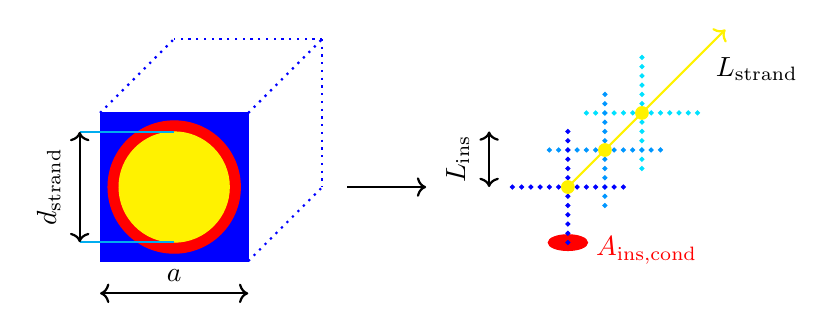
\begin{tikzpicture}[scale = 1]
        \filldraw[blue] (-0.941,-0.941) rectangle (0.941,0.941);
        \filldraw[red] (0,0) circle (0.7+0.07*2);
        \filldraw[yellow] (0,0) circle (0.7);
        \draw[thick, cyan] (-0.8*1.5,0.7) -- (0,0.7);
        \draw[thick, cyan] (-0.8*1.5,-0.7) -- (0,-0.7);
        \draw[black, thick, <->] (-0.75*1.6,0.7) -- (-0.75*1.6,-0.7);
        \node[scale = 1, rotate=90] at (-1.1*1.45, 0) {$d_\text{strand}$};
        \draw[thick,<->] (-0.941,-0.9*1.5) -- (0.941,-0.9*1.5);
        \node[scale = 1] at (0, -0.7*1.6) {$a$};
        \draw[thick, dotted, blue] (0.941,0.941) -- (2*0.941,2*0.941);
        \draw[thick, dotted, blue] (-0.941,0.941) -- (0,2*0.941);
        \draw[thick, dotted, blue] (0.941,-0.941) -- (2*0.941,0);
        \draw[thick, dotted, blue] (2*0.941,2*0.941) -- (2*0.941,0);
        \draw[thick, dotted, blue] (2*0.941,2*0.941) -- (0,2*0.941);
        % ellipse for insulation area
        \filldraw[red] (5.0,-5.646/8) ellipse (0.25cm and 0.1cm);
        \node[scale = 1, red] at (6.0, -5.646/8-0.1) {$A_\text{ins,cond}$};
        % third insulation layer
        \definecolor{blue_third_layer}{RGB}{0,225,255}
        \foreach \x in {-5.646,-4.705,...,5.646} 
            \filldraw[blue_third_layer] (5.0+2*0.4705,\x/8+2*0.4705) circle (0.025);
        \foreach \x in {-5.646,-4.705,...,5.646} 
            \filldraw[blue_third_layer] (5.0+\x/8+2*0.4705,2*0.4705) circle (0.025);
        % second insulation layer
        \definecolor{blue_second_layer}{RGB}{0,150,255}
        \foreach \x in {-5.646,-4.705,...,5.646} 
            \filldraw[blue_second_layer] (5.0+0.4705,\x/8+0.4705) circle (0.025);
        \foreach \x in {-5.646,-4.705,...,5.646} 
            \filldraw[blue_second_layer] (5.0+\x/8+0.4705,0.4705) circle (0.025);
        % first insulation layer
        \definecolor{blue_first_layer}{RGB}{0,0,255}
        \foreach \x in {-5.646,-4.705,...,5.646} 
            \filldraw[blue_first_layer] (5.0,\x/8) circle (0.025);
        \foreach \x in {-5.646,-4.705,...,5.646} 
            \filldraw[blue_first_layer] (5.0+\x/8,0) circle (0.025);
        % strand nodes
        \draw[thick, yellow, ->] (5.0,0) -- (7.0,2.0);
        \foreach \t in {0.0,0.4705,...,1.4115}
            \filldraw[yellow] (5.0+\t,\t) circle (0.08);
        \node[scale = 1] at (7.4, 1.5) {$L_\text{strand}$};    
        \draw[thick, black, <->] (4,0) -- (4,5.646/8);
        \node[scale = 1, rotate=90] at (3.6, 5.646/16) {$L_\text{ins}$}; 
        % draw arrow
        \draw[thick, black, ->] (2.2,0) -- (3.2,0);
    \end{tikzpicture}
    \caption{3-dimensional translation of a 1D+1D strand domain}
    \label{fig: 1d_strand_geometry_with_insulation}
\end{figure}




Insulation dimensions:

\begin{equation}
    A_\text{ins} = a^2 - \frac{\pi d_\text{strand}^2}{4}
\end{equation}

\begin{equation}
    p_\text{avg} = \frac{4 a + \pi d_\text{strand}}{2} 
\end{equation}

\begin{equation}
    L_\text{ins} = \frac{A_\text{ins}}{p_\text{avg}}
\end{equation}

\begin{equation}
    A_\text{ins,cond} = \frac{\frac{1}{4} A_\text{ins} ~ L_{winding}}{L_\text{ins}}
\end{equation}


\begin{figure}[h!]
\centering
    \begin{tikzpicture}
        \begin{axis}[
          no markers,
          width=0.7\linewidth, 
          height = 4.5cm,
          xlabel={$L_\text{strand},~\text{m}$},
          ylabel={$T,~\text{K}$},
          xmin=0.0,
          ymin=0.0,
          xmax=1.0
          ]
        %   Initial temperature curve
          \addplot[smooth, black] table[x=posx,y=t_0_0_ans,col sep=comma] {sections/1D_quench_modelling/figures/results_with_insulation/10ms_1e4elemsf2_2ins_insTem_in.csv};
          
        %   COMSOL plots
          \addplot[smooth, red] table[x=posx,y=t_0_03_com,col sep=comma] {sections/1D_quench_modelling/figures/results_with_insulation/10ms_1e4elemsf2_2ins_insTem_in.csv};
          \addplot[smooth, red] table[x=posx,y=t_0_06_com,col sep=comma] {sections/1D_quench_modelling/figures/results_with_insulation/10ms_1e4elemsf2_2ins_insTem_in.csv};
          \addplot[smooth, red] table[x=posx,y=t_0_1_com,col sep=comma] {sections/1D_quench_modelling/figures/results_with_insulation/10ms_1e4elemsf2_2ins_insTem_in.csv};

        %   ANSYS plots
          \addplot[smooth, blue] table[x=posx,y=t_0_03_ans,col sep=comma] {sections/1D_quench_modelling/figures/results_with_insulation/10ms_1e4elemsf2_2ins_insTem_in.csv};
          \addplot[smooth, blue] table[x=posx,y=t_0_06_ans,col sep=comma] {sections/1D_quench_modelling/figures/results_with_insulation/10ms_1e4elemsf2_2ins_insTem_in.csv};
          \addplot[smooth, blue] table[x=posx,y=t_0_1_ans,col sep=comma] {sections/1D_quench_modelling/figures/results_with_insulation/10ms_1e4elemsf2_2ins_insTem_in.csv};
          
        \end{axis}
    \end{tikzpicture}
    \caption{Temperature distribution calculated in COMSOL (red) and ANSYS (blue) for three time frames: $t=\{0.03, 0.06, 0.1\}$ s.}
    \label{fig: 1d_with_insulation_temp_along_strand_comparison}
\end{figure}

\begin{figure}[h!]
\centering
    \begin{tikzpicture}
        \begin{axis}[
          width=0.7\linewidth, 
          height = 4.5cm,
          xlabel={$L_\text{strand},~\text{m}$},
          ylabel={Relative error, \%},
          xmin=0.0,
          xmax=1.0
          ]
          \addplot[blue, mark=*] table[x=posx,y=error_0_1,col sep=comma] {sections/1D_quench_modelling/figures/results_with_insulation/10ms_1e4elemsf2_2ins_insTem_in_error.csv};
        \end{axis}
    \end{tikzpicture}
    \caption{Relative error along the strand for $t=0.1~\text{s}$.}
    \label{fig: ans_comsol_comparison_f_2_2_with_insulation}
\end{figure}
 
 
% QUENCH VELOCITY MODELLING
\clearpage
\section{Quench Velocity Modelling}
\label{section:quench_velocity_modelling}

When quench occurs, one can notice that the point at which the cable transforms from superconducting to normal state propagates with time. This point remains at the critical temperature, $T_\text{c}$ for a given magnetic field strength. For the purpose of quench velocity modelling, the interesting feature of this point is how it changes its position in time, as described in Fig. \ref{fig:modelling_approach}. Depending on the electro-magneto-thermal conditions at which quench occurs, quench velocity can remain constant or change in time. 

\begin{figure}[H]
\centering
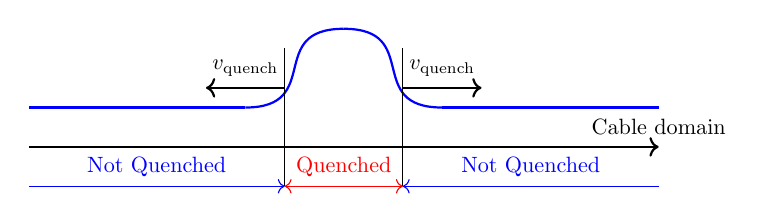
\begin{tikzpicture}[scale = 1]
\draw [thick, ->] (0.0,0.0) -- (8.0,0);

\draw [thick, blue] (0.0,0.5) -- (2.75,0.5);
\draw [thick, blue] (5.25,0.5) -- (8.0,0.5);

\draw [thick, blue] (2.75,0.5) .. controls +(0:1cm) and +(180:1cm) .. (4.0,1.5);
\draw [thick, blue] (4.0,1.5) .. controls +(0:1cm) and +(180:1cm) .. (5.25,0.5);

\draw [thin] (3.25,-0.5) -- (3.25,1.25);
\draw [thin] (4.75,-0.5) -- (4.75,1.25);

\draw [thick, ->] (4.75,0.75) -- (5.75,0.75);
\draw [thick, ->] (3.25,0.75) -- (2.25,0.75);

\draw [thin, red, <->] (3.25,-0.5) -- (4.75,-0.5);
\draw [thin, blue, ->] (0.0,-0.5) -- (3.25,-0.5);
\draw [thin, blue, <-] (4.75,-0.5) -- (8.0,-0.5);

\node[scale = 0.8] [color = red] at (4.0,-0.25) {Quenched};
\node[scale = 0.8] [color = blue] at (1.625,-0.25) {Not Quenched};
\node[scale = 0.8] [color = blue] at (6.375,-0.25) {Not Quenched};

\node[scale = 0.8] at (5.25,1.0) {$v_\text{quench}$};
\node[scale = 0.8] at (2.75,1.0) {$v_\text{quench}$};
\node[scale = 0.8] at (8.0,+0.25) {Cable domain};

\end{tikzpicture}
\caption{Quench velocity approach.}
\label{fig:modelling_approach}
\end{figure}

Quench velocity can be approximated with analytic formulas. They are usually a function of current density, material properties of the winding and temperature gradient around the quench front. The quench velocity in ITER applications is mainly estimated based on~\cite{MIT_phd_thesis}. For superconducting accelerator magnets, Wilson's formula is more applicable if cooling with helium is not considered \cite[p.~206]{wilson1987superconducting}, as described below
\begin{equation}
    v_\text{quench}=\frac{J}{\gamma C}\sqrt{\frac{\rho k}{T_\text{s}-T_\text{0}}},
    \label{eqn:Wilson_quench_velocity_formula}
\end{equation}
where $T_\text{s}$ -- critical temperature,
$T_\text{0}$ -- coolant temperature,
$\rho$ -- resistivity averaged over the conductor volume,
$J$ -- current density averaged over the conductor volume,
$k$ -- thermal conductivity averaged over the conductor unit cell,
$C$ -- specific heat averaged over the conductor unit cell,
$\gamma$ -- conductor density.

In standard heat conduction multi-dimensional quench problem, the solver tries to find a temperature distribution in a given space and time. It is usually computationally costly because one should cope with a temperature distribution being steep at the level of the quench front. Due to high material non-linearities at cryogenic temperatures, in order to accurately solve temperature distribution in the entire region of the cable, one should refine mesh or decrease the simulation time step (up to the order of a $\mu$s). In both cases the simulation time usually becomes excessively long. All material properties used in scope of the thesis are presented in Appendix \ref{appendix_material_properties_description}.

As presented in Fig. \ref{fig:modelling_approach}, the quenched and non-quenched regions in a superconducting cable have different but relatively uniform temperature distributions. Therefore, the solution of heat conduction equation in two of these regions is easier to solve than at the quench front where both regions meet with their already importantly different material properties such as thermal conductivity or specific heat capacity. The method simplifying the thermal quench modelling, called quench velocity method, bases on predicting quench velocity by an outsourced external routine. Such an approach allows one to have the quench wave explicitly solved and, therefore, an accurate solution of temperature distribution at the quench front is not required. As a result, the mesh refinement along the coil length is not needed anymore and the numerical model is of a smaller size to be solved. Therefore, the numerical model still calculates the heat balance equation but with a fixed and relatively coarse mesh along the coil of a magnet. 
 
\begin{figure}[H]
\centering
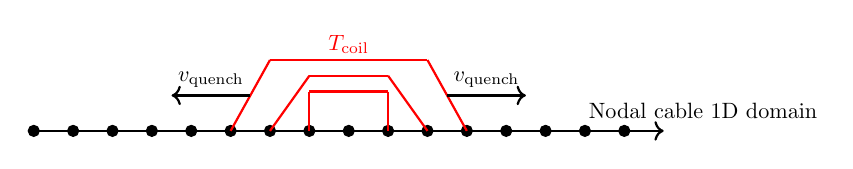
\begin{tikzpicture}[scale = 1]
\draw [thick, ->] (0.0,0.0) -- (8.0,0);
\foreach \t in {0,0.5,1,...,7.5}
\filldraw[black] ({\t},0) circle (2pt);
\node[scale = 0.8] at (8.5,0.25) {Nodal cable 1D domain};
\draw [thick, red] (3.5,0) -- (3.5,0.5);
\draw [thick, red] (3.5,0.5) -- (4.5,0.5);
\draw [thick, red] (4.5,0.5) -- (4.5,0);
\draw [thick, red] (3,0) -- (3.5,0.7);
\draw [thick, red] (3.5,0.7) -- (4.5,0.7);
\draw [thick, red] (4.5,0.7) -- (5,0);
\draw [thick, red] (2.5,0) -- (3,0.9);
\draw [thick, red] (3,0.9) -- (5,0.9);
\draw [thick, red] (5,0.9) -- (5.5,0);
\draw [thick, ->] (5.25,0.45) -- (6.25,0.45);
\node[scale = 0.8] at (5.75,0.65) {$v_\text{quench}$};
\draw [thick, ->] (2.75,0.45) -- (1.75,0.45);
\node[scale = 0.8] at (2.25,0.65) {$v_\text{quench}$};
\node[scale = 0.8, red] at (4,1.1) {$T_\text{coil}$};
\end{tikzpicture}
\caption{Schematic temperature propagation with quench velocity modelling.}
\label{fig:modelling_approach}
\end{figure}

Solving quench propagation by means of quench velocity method assumes that, while  simulating the heat propagation during quench, the quench front velocity is known and estimated separately beforehand. The quench velocity can be:
\begin{itemize}
\item assumed constant,
\item based on available measurements,
\item calculated analytically,
\item calculated numerically.
\end{itemize}

In numerical thermal 3D problem, there are two phenomena to be analysed important for the quench simulations: $(i)$~longitudinal propagation of quench, $(ii)$~transverse propagation of quench across the insulation between separate windings of the coil. Only the \nth{1} part is solved by means of a quench velocity - based thermal model. In order to conduct a 3D thermal analysis using quench velocity method, the simulation tools listed below need to be developed: 
\begin{enumerate}
\item electro-thermal model simulating longitudinal quench propagation
\item thermal model simulating transverse thermal propagation across insulation
\item algorithm mapping multidimensional winding geometry onto 1D coil
\item algorithm calculating quench velocity
\item algorithm assigning node numbers to quench position varying in time
\item algorithm detecting new quenches across multiple windings
\end{enumerate}

ANSYS environment was chosen to perform the electro-thermal and thermal analyses. The external algorithms are prepared in Python. This chapter describes all the aforementioned algorithms as well as their implementation in Python-ANSYS coupling.

\subsection{Quench Velocity Algorithm}
\label{subsection:quench_velocity_algorithm}

This part of the chapter describes how the quench velocity method is applied in ANSYS simulations via Python script. In order to distinguish the quenched zone from the non-quenched one, the superconducting cable is divided into two domains as presented in Fig. \ref{fig:ansys_material_assignment}. The non-quenched part is characterised by nearly zero-resistivity for the sake of numerical stability whereas the quenched cable has nonlinear resistivity properties of copper. The material properties are reassigned at each time step as the quench propagates in ANSYS model.

\begin{figure}[H]
\centering
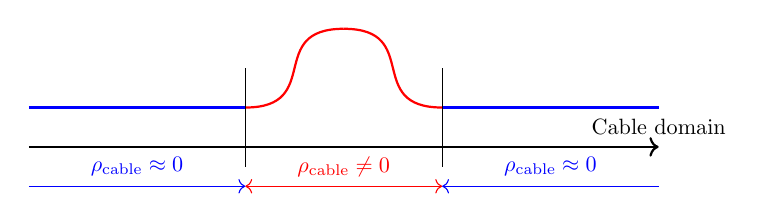
\begin{tikzpicture}[scale = 1]
\draw [thick, ->] (0.0,0.0) -- (8.0,0);
\draw [thick, blue] (0.0,0.5) -- (2.75,0.5);
\draw [thick, blue] (5.25,0.5) -- (8.0,0.5);
\draw [thick, red] (2.75,0.5) .. controls +(0:1cm) and +(180:1cm) .. (4.0,1.5);
\draw [thick, red] (4.0,1.5) .. controls +(0:1cm) and +(180:1cm) .. (5.25,0.5);
\draw [thin] (2.75,-0.25) -- (2.75,1.0);
\draw [thin] (5.25,-0.25) -- (5.25,1.0);
\draw [thin, red, <->] (2.75,-0.5) -- (5.25,-0.5);
\draw [thin, blue, ->] (0.0,-0.5) -- (2.75,-0.5);
\draw [thin, blue, <-] (5.25,-0.5) -- (8.0,-0.5);
\node[scale = 0.8] [color = red] at (4.0,-0.25) {$\rho_\text{cable} \neq 0$};
\node[scale = 0.8] [color = blue] at (1.375,-0.25) {$\rho_\text{cable} \approx 0$};
\node[scale = 0.8] [color = blue] at (6.625,-0.25) {$\rho_\text{cable} \approx 0$};
\node[scale = 0.8] at (8.0,+0.25) {Cable domain};
\end{tikzpicture}
\caption{ANSYS cable domain assignment.}
    \label{fig:ansys_material_assignment}
\end{figure}

As described at the beginning of the chapter, the quench velocity can be: $(a)$ assumed constant, $(b)$ based on available measurements, $(c)$ calculated numerically, $(d)$ calculated analytically according to quench velocity equations available in literature. The first 3 above-mentioned methods to calculate quench velocity would require one-directional exchange of signals between Python and ANSYS, as described in \ref{fig:unidirectional_coupling_scheme}. The initial quench length should be assumed in Python when starting the quench velocity algorithm. Then, ANSYS environment is provided with a Python quench front position from the previous communication point $T_{j-1}$ and calculates temperature distribution in the current communication point $T_j$.

If quench velocity is analysed by means of analytic formula (like in the \nth{4} case), quench velocity algorithm should be a bidirectional exchange of signals in form of weak coupling, as presented in Fig. \ref{fig:bidirectional_coupling_scheme}. In such a case, Python script is provided with the data from ANSYS at point $T_j$ to estimate quench velocity at point $T_{j-1}$ up to the point $T_j$. The line which describes the information direction is marked in red in Fig. \ref{fig:bidirectional_coupling_scheme}.

Between the Python time steps, ANSYS solves the problem with an automatic time step where the minimum and the maximum time step is defined by a user. For the purpose of this thesis, the Python script was developed to calculate quench velocity assuming that it constant or it is calculated numerically (case a and c). The creation of a numerical map for the quench velocity will be further described in chapter \ref{section:skew_quadrupole_quench_detection_analysis}. This method is used for quench velocity modelling of a skew quadrupole.

\begin{figure}[H]
\centering
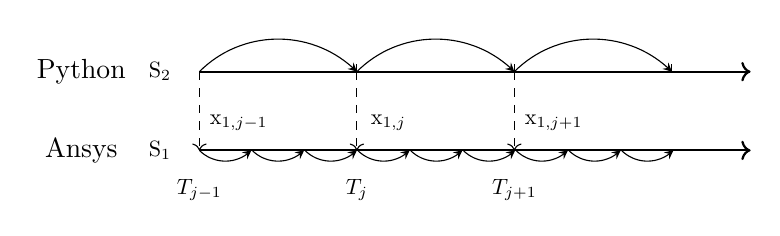
\begin{tikzpicture}[scale = 1]
\draw[thick,->] (0,1) -- (7,1);
\draw (2, 1) -- (2, 1.1);
\draw (4, 1) -- (4, 1.1);
\draw (6, 1) -- (6, 1.1);
\foreach \t in {1,3,5}
\draw [-stealth, bend angle=45, bend left, color = black]  ({\t-1},1) to (\t+1,1);
\draw[thick,->] (0,0) -- (7,0);
\draw (2, 1) -- (2, 1.1);
\draw (4, 1) -- (4, 1.1);
\draw (6, 1) -- (6, 1.1);
\foreach \t in {0.66,1.33,...,6.33}
\draw [-stealth, bend angle=45, bend right]  ({\t-0.66},0) to (\t,0);
\node[scale = 0.8] at (0, -0.5) {$T_{j-1}$};
\node[scale = 0.8] at (2,-0.5) {$T_j$};
\node[scale = 0.8] at (4,-0.5) {$T_{j+1}$};
\draw[dashed, ->] (0,1) -- (0,0);
\draw[dashed, ->] (2,1) -- (2,0);
\draw[dashed, ->] (4,1) -- (4,0);
\node[scale = 0.8] at (-0.5, 0) {$\text{S}_1$};
\node[scale = 0.8] at (-0.5, 1) {$\text{S}_2$};
\node[scale = 0.8] at (0.5, 0.35) {$\text{x}_{1,j-1}$};
\node[scale = 0.8] at (2.4, 0.35) {$\text{x}_{1,j}$};
\node[scale = 0.8] at (4.5, 0.35) {$\text{x}_{1,j+1}$};
\node[color = black] at (-1.5,1.0)	{Python};
\node at (-1.5,0)	{Ansys};
\end{tikzpicture}
\caption{Schematic representation of unidirectional coupling between ANSYS and external Python code.}
\label{fig:unidirectional_coupling_scheme}
\end{figure}

\begin{figure}[H]
\centering
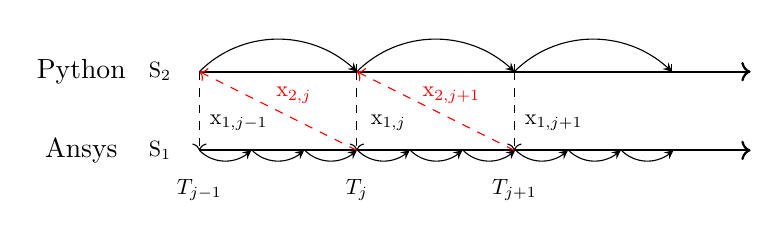
\begin{tikzpicture}[scale = 1]
\draw[thick,->] (0,1) -- (7,1);
\draw (2, 1) -- (2, 1.1);
\draw (4, 1) -- (4, 1.1);
\draw (6, 1) -- (6, 1.1);
\foreach \t in {1,3,5}
\draw [-stealth, bend angle=45, bend left, color = black]  ({\t-1},1) to (\t+1,1);
\draw[thick,->] (0,0) -- (7,0);
\draw (2, 1) -- (2, 1.1);
\draw (4, 1) -- (4, 1.1);
\draw (6, 1) -- (6, 1.1);
\foreach \t in {0.66,1.33,...,6.33}
\draw [-stealth, bend angle=45, bend right]  ({\t-0.66},0) to (\t,0);
\node[scale = 0.8] at (0, -0.5) {$T_{j-1}$};
\node[scale = 0.8] at (2,-0.5) {$T_j$};
\node[scale = 0.8] at (4,-0.5) {$T_{j+1}$};
\draw[dashed, ->] (0,1) -- (0,0);
\draw[dashed, ->] (2,1) -- (2,0);
\draw[dashed, ->] (4,1) -- (4,0);
\draw[dashed, red, ->] (2,0) -- (0,1);
\draw[dashed, red, ->] (4,0) -- (2,1);
\node[scale = 0.8] at (-0.5, 0) {$\text{S}_1$};
\node[scale = 0.8] at (-0.5, 1) {$\text{S}_2$};
\node[scale = 0.8] at (0.5, 0.35) {$\text{x}_{1,j-1}$};
\node[scale = 0.8] at (2.4, 0.35) {$\text{x}_{1,j}$};
\node[scale = 0.8] at (4.5, 0.35) {$\text{x}_{1,j+1}$};
\node[scale = 0.8, red] at (1.2, 0.7) {$\text{x}_{2,j}$};
\node[scale = 0.8, red] at (3.2, 0.7) {$\text{x}_{2,j+1}$};
\node[color = black] at (-1.5,1.0)	{Python};
\node at (-1.5,0)	{Ansys};
\end{tikzpicture}
\caption{Schematic representation of bidirectional coupling between ANSYS and external Python code.}
\label{fig:bidirectional_coupling_scheme}
\end{figure}

Provided that data exchange between Python module and ANSYS occurs at communication times $T_j$, the quench velocity algorithm is solved as described in Algorithm \ref{alg:weak_coupling}.

\begin{algorithm}
  \caption{Weak Coupling between ANSYS and Python environment}
  \label{alg:weak_coupling}
  \begin{algorithmic}[1]
    \STATE assume initial quench position $x_{1,j-1}$ 
    \STATE \textbf{for} $j=1,2,...,N$ \textbf{do}
    \STATE \hspace{0.5cm} solve temperature distribution at time $T_j$
    \STATE \hspace{0.5cm} extrapolate ANSYS results $x_{2,j}$ to Python step $T_{j-1}$ (bidirectional case from Fig. \ref{fig:bidirectional_coupling_scheme})
    \STATE \hspace{0.5cm} estimate new quench position $x_{1,j}$ for each existing quench front
    \STATE \hspace{0.5cm} assign quench position $x_{1,j}$ to new nodes for ANSYS time step $T_j$
  \end{algorithmic}
\end{algorithm}


\subsection{Quench Velocity Benchmarking}
\label{subsection:quench_velocity_benchmarking}

The aim of this section is to compare the proposed quench velocity - based analysis with a standard heat balance equation modelling in ANSYS. The elements to compare are: 
\begin{itemize}
    \item number of nodes,
    \item time step applied,
    \item relative error, 
    \item computing time.
\end{itemize}

The \nth{1} step is to conduct a heat balance equation - based analysis. It will serve for two purposes: ($i$) reference model for relative error, ($ii$) quench velocity value to be used in quench velocity - based model. The \nth{2} stage aims at conducting quench velocity - based simulations with quench velocity value obtained from 1D numerical heat balance equation - based models. 

In this section, all material properties are based on NIST standards described in Appendix \ref{appendix_material_properties_description}. The analysis is conducted for two cases separately: 
\begin{itemize}
    \item 1D strand analysis without insulation layer,
    \item 1D strand analysis with an external insulation layer.
\end{itemize}



% ALGORITHMS AND PYTHON IMPLEMENTATION
\clearpage
\section{Algorithms}
\label{section:algorithms}

\subsection{Multidimensional Mapping Algorithm}
\label{subsection:multidimensional_mapping_algorithm}

The algorithm mapping multi-strand and multi-dimensional magnet geometries is explained in this section. Superconducting accelerator magnets are made from a strand or a bunch of strands, e.g. Rutherford cable\footnote{Rutherford cable is a type of an electrical cable used in superconducting technologies reducing Eddy current effects during the ramp up.}, wound multiple times in a certain pattern. Creating a CAD geometry where a~single strand domain is wound $n$ times would be a~complicated task. Therefore, every winding of the strand is considered as a~separate domain, as shown in Fig. \ref{fig:winding_geom_scheme}. The end of the windings marked in red are coupled with the neighbouring ones thermally and electrically, i.e. they are characterised by the same temperature and voltage. With such an approach, one can easily create multi-strand magnet geometries. Moreover, by specifying which windings are couple together, with the same numerical domain, one can also analyse magnets with different winding schemes.

\begin{figure}[H]
\centering
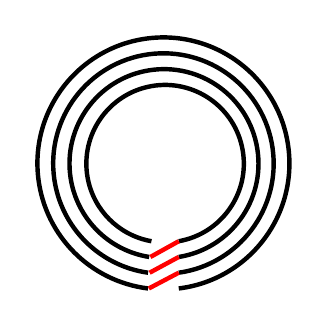
\begin{tikzpicture}[scale = 1]

\draw [ultra thick] (0,0) arc (-80:260:1);
\draw [ultra thick] (0,-0.2) arc (-81:261:1.2);
\draw [ultra thick] (0,-0.4) arc (-82:262:1.4);
\draw [ultra thick] (0,-0.6) arc (-83:263:1.6);

\draw [ultra thick, red] (0,0) -- (-0.36,-0.2);
\draw [ultra thick, red] (0,-0.2) -- (-0.37,-0.4);
\draw [ultra thick, red] (0,-0.4) -- (-0.38,-0.6);

\end{tikzpicture}
\caption{Domain representation with multiple windings.}
\label{fig:winding_geom_scheme}
\end{figure}

As illustrated in Fig.~\ref{fig: 3d_coil_illustation_with_2d_b_field}, a multi-strand domain is subjected to a varying magnetic field across the different windings~$i$. Since it is assumed that the coil is infinitely long, the magnetic field is calculated from a 2D model of a central magnet cross-section. 

\begin{figure}[H]
    \centering
    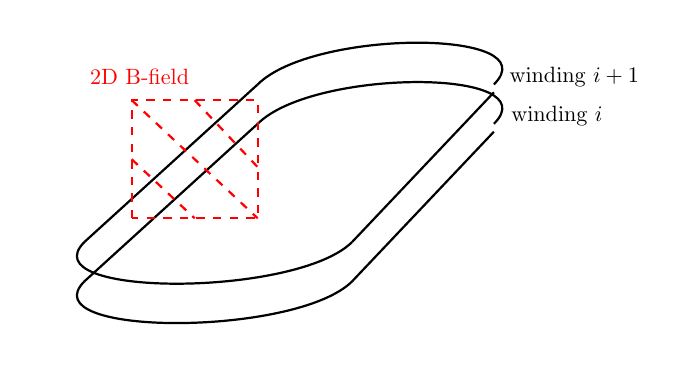
\begin{tikzpicture}[scale = 1]
        
        \foreach \y in {0,0.5} 
        \draw[thick,  black] (0.2,\y) -- (2,\y+1.9);
        
        \foreach \y in {0,0.5} 
        \draw[thick, black] (.2,\y) .. controls +(45:-1cm) and +(45:-1cm) .. (-3.2,\y);
        
        \foreach \y in {0,0.5} 
        \draw[thick,  black] (-3.2,\y) -- (-1,\y+2.0);
        
        \foreach \y in {0,0.5} 
        \draw[thick, black] (-1,\y+2) .. controls +(45:1cm) and +(45:1cm) .. (2,\y+2);
        
        \draw[thick, dashed, red] (-2.6,0.8) rectangle (-1.0,2.3);
        \draw[thick, dashed, red] (-2.6,1.55) -- (-1.8, 0.8);
        \draw[thick, dashed, red] (-2.6,2.3) -- (-1.0, 0.8);
        \draw[thick, dashed, red] (-1.8,2.3) -- (-1.0, 1.45);
        
        \node[scale = 0.8] at (2.8,2.1) {winding $i$};
        \node[scale = 0.8] at (3.02,2.6) {winding $i+1$};
        
        \node[red, scale = 0.8] at (-2.5,2.6) {2D B-field};
        
    \end{tikzpicture}
    \caption{Schematic of an assignment of a magnetic field to a multi-strand domain.}
    \label{fig: 3d_coil_illustation_with_2d_b_field}
\end{figure}

The different values of magnetic field are assigned to different windings, as shown in Fig.~\ref{fig:ansys_python_mapping scheme}. Since a different value of a magnetic field is assigned to each winding, every strand is characterised by different thermal and electrical material properties. Then, the multi-strand geometry is translated into a realistic one-dimensional cable with a length equal to the length of all the windings of a magnet. Each part of this coil length, $L_\text{coil, 1D}$ representing one winding is characterised by a different value of a magnetic field field~$B_\text{n}$.

\begin{figure}[H]
\centering
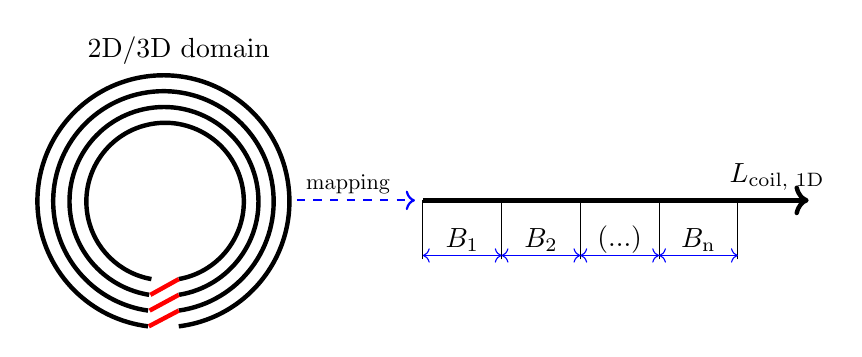
\begin{tikzpicture}[scale = 1]
\draw [ultra thick] (0,0) arc (-80:260:1);
\draw [ultra thick] (0,-0.2) arc (-81:261:1.2);
\draw [ultra thick] (0,-0.4) arc (-82:262:1.4);
\draw [ultra thick] (0,-0.6) arc (-83:263:1.6);
\draw [ultra thick, red] (0,0) -- (-0.36,-0.2);
\draw [ultra thick, red] (0,-0.2) -- (-0.37,-0.4);
\draw [ultra thick, red] (0,-0.4) -- (-0.38,-0.6);
\node[scale = 1.0] at (0,2.9) {2D/3D domain};
\draw [thick, dashed, blue, ->] (1.5,1) -- (3,1);
\node[scale = 0.8] at (2.15,1.2) {mapping};
\draw [ultra thick, ->] (3.1,1) -- (8,1);
\foreach \t in {3.1, 4.1, ..., 7.1}
\draw [thin] ({\t},0.25) -- ({\t},1);
\foreach \t in {3.1, 4.1, ..., 6.1}
\draw [thin, blue, <->] ({\t},0.3) -- ({\t+1},0.3);
\node[scale = 1.0] at (3.6,0.5) {$B_1$};
\node[scale = 1.0] at (4.6,0.5) {$B_2$};
\node[scale = 1.0] at (5.6,0.5) {(...)};
\node[scale = 1.0] at (6.6,0.5) {$B_\text{n}$};
\node[scale = 1.0] at (7.6,1.3) {$L_\text{coil, 1D}$};
\end{tikzpicture}
\caption{Multidimensional mapping scheme.}
\label{fig:ansys_python_mapping scheme}
\end{figure}

In Chapter~\ref{chapter: 1d_quench_propagation_modelling}, a uniform temperature was assumed in the cross-section of a strand which allowed for modelling the coil with a 1D longitudinal nodal domain. If such an assumption is not made, the composite strand is modelled with 2D or 3D nodal elements. As presented in Fig.~\ref{fig: mesh_generation_in_multidimensional_case}, the mesh is generated by specifying 2D nodal planes  uniformly distributed in a longitudinal direction of the coil. The planes are always perpendicular to the normal vector $\vec{n}$ of a directional spline. 

\begin{figure}[H]
    \centering
    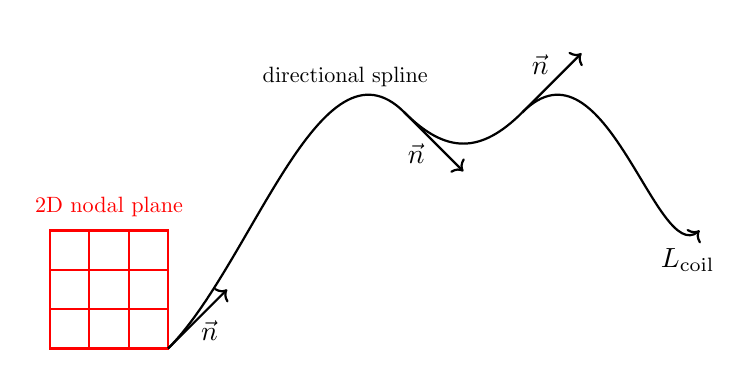
\begin{tikzpicture}[scale = 1.5]
        
        \draw[thick, red] (-1,1) rectangle (0,0);
        \draw[thick, red] (-1,1/3) -- (0,1/3);
        \draw[thick, red] (-1,2/3) -- (0,2/3);
        \draw[thick, red] (-1/3,0) -- (-1/3,1);
        \draw[thick, red] (-2/3,0) -- (-2/3,1);
        
        \draw[thick, black] (0,0) .. controls +(45:1cm) and +(135:1cm) .. (2,2);
        \draw[thick, black] (2,2) .. controls +(135:-0.5cm) and +(45:-0.5cm) .. (3,2);
        \draw[thick, black, ->] (3,2) .. controls +(45:1cm) and +(45:-0.5cm) .. (4.5,1);
        
        \draw[thick, black, ->] (0,0) -- (0.5,0.5);
        \draw[thick, black, ->] (2,2) -- (2.5,1.5);
        \draw[thick, black, ->] (3,2) -- (3.5,2.5);

        \node[red, scale=0.8] at (-0.5,1.2) {2D nodal plane};
        \node[black, scale=0.8] at (1.5,2.3) {directional spline};
        \node[black] at (0.35,0.15) {$\vec{n}$};
        \node[black] at (2.1,1.65) {$\vec{n}$};
        \node[black] at (3.15,2.4) {$\vec{n}$};
        \node[scale = 1.0] at (4.4,0.75) {$L_\text{coil}$};
        
    \end{tikzpicture}
    \caption{Multidimensional mesh generation in mapping algorithm.}
    \label{fig: mesh_generation_in_multidimensional_case}
\end{figure}

As illustrated in Fig.~\ref{fig:ansys_python_mapping scheme_nodes}, 2D nodal planes~$P_\text{n}$ are packed into a set of imaginary nodes~$N_\text{n}$ in the external routine calculating the propagation of quench. Each imaginary node~$P$ represents one plane~$N$. The position of the imaginary node~$N$ in space is an average position of all the nodes belonging to the plane~$P$. The creation of imaginary nodes serves for facilitating the assignment of quenched zones in time by an external routine. This process is performed in order to estimate the quench propagation only in the longitudinal direction.

\begin{figure}[H]
\centering
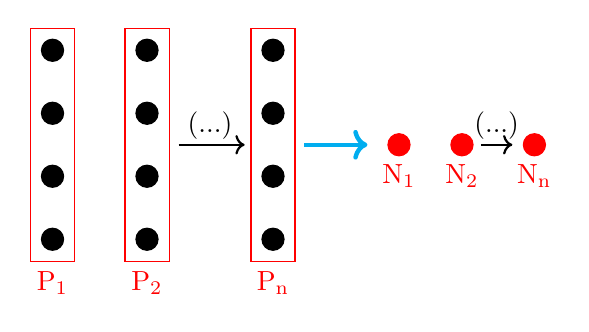
\begin{tikzpicture}[scale = 0.8]

    \foreach \t in {0,1,...,3}
    \filldraw[black] (0,{\t}) circle (5pt);
    \foreach \t in {0,1,...,3}
    \filldraw[black] (1.5,{\t}) circle (5pt);
    \foreach \t in {0,1,...,3}
    \filldraw[black] (3.5,{\t}) circle (5pt);
    \draw[red] (-0.35,-0.35) rectangle (0.35,3.35);
    \draw[red] (1.15,-0.35) rectangle (1.85,3.35);
    \draw[red] (3.15,-0.35) rectangle (3.85,3.35);
    \draw[thick,->] (2,1.5) -- (3.05,1.5);
    
    \node at (2.5, 1.8) {(...)};
    \node[red] at (0, -0.7) {$\text{P}_1$};
    \node[red] at (1.5, -0.7) {$\text{P}_2$};
    \node[red] at (3.5, -0.7) {$\text{P}_\text{n}$};
    
    \draw[ultra thick,->, cyan] (4,1.5) -- (5,1.5);
    \filldraw[red] (5.5,1.5) circle (5pt);
    \filldraw[red] (6.5,1.5) circle (5pt);
    \draw[thick,->] (6.8,1.5) -- (7.3,1.5);
    \filldraw[red] (7.65,1.5) circle (5pt);
    
    \node at (7.05, 1.8) {(...)};
    \node[red] at (5.5, 1) {$\text{N}_1$};
    \node[red] at (6.5, 1) {$\text{N}_2$};
    \node[red] at (7.65, 1) {$\text{N}_\text{n}$};

\end{tikzpicture}
\caption{Schematic of node assignment to imaginary nodes.}
    \label{fig:ansys_python_mapping scheme_nodes}
\end{figure}

\subsection{Node Searching Algorithm}
\label{subsection:node_searching_algorithm}

Regardless the manner how the quench velocity is calculated, the external routine will always understand the quench length as if it was a continuous function of time. Therefore, it is expected that the calculated quench position~$L$ in a given time will differ from the available positions of a discrete meshed geometry in a numerical solver. Therefore, it is important to create an algorithm assigning the nodes to the quenched and non-quenched zones in a discretised domain.

The quench zone assignment algorithm is presented in Fig. \ref{fig:node_search_algo}. It searches the node $N_\text{search}$ whose geometric position is below the assumed error,~$\epsilon$ compared to the quench length $L$ calculated on the side of an external routine estimating quench velocity. At each time step the algorithm checks whether $N_\text{search}$ is within the space $N$ and ${N+x}$ when jump search is considered. In case of a dense mesh, the step control doubles if the right zone ${[N+(a-1)x, N+ax]}$ is not found after 5 iterations. When the node space ${[N+(a-1)x, N+ax]}$ contains the searched node, it uses the binary search to find the node fulfilling the condition ${\mid L(N_\text{search}) - L \mid \geq \epsilon}$. 

\begin{figure}[H]
\centering
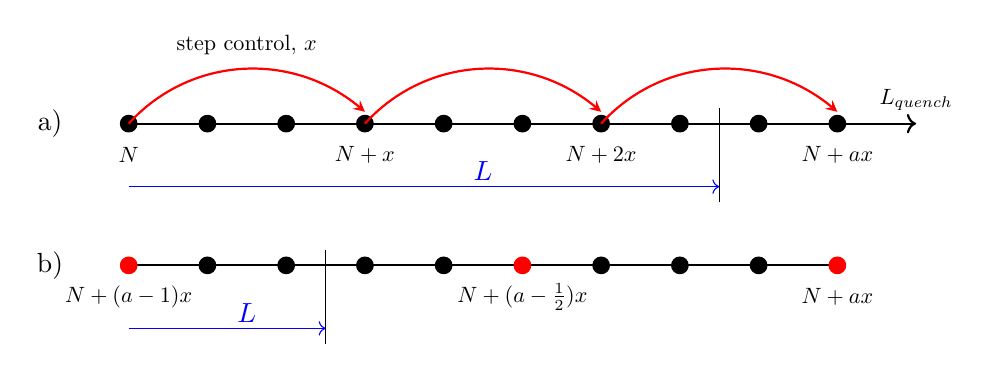
\begin{tikzpicture}[scale = 1]
\draw[thick,->] (0,1) -- (10,1);
\foreach \t in {0,1,...,9}
\filldraw[black] ({\t},1) circle (3pt);
\foreach \t in {1,4,7}
\draw [thick, -stealth, bend angle=45, bend left, color = red]  ({\t-1},1) to (\t+2,1.15);
\node[scale = 0.8] at (1.5, 2) {step control, $x$};
\node[scale = 0.8] at (0, 0.6) {$N$};
\node[scale = 0.8] at (3, 0.6) {$N+x$};
\node[scale = 0.8] at (6, 0.6) {$N+2x$};
\node[scale = 0.8] at (9, 0.6) {$N+ax$};
\node[scale = 0.8] at (10, 1.3) {$L_{quench}$};
\draw[thin, blue, ->] (0,0.2) -- (7.5,0.2);
\draw[thin, black] (7.5,0) -- (7.5,1.2);
\node[scale = 1, blue] at (4.5, 0.4) {$L$};
\node at (-1, 1) {a)};

\draw[thick] (0,-0.8) -- (9,-0.8);
\foreach \t in {1,2,3,4,6,7,8}
\filldraw[black] ({\t},-0.8) circle (3pt);
\foreach \t in {0,5,9}
\filldraw[red] ({\t},-0.8) circle (3pt);
\node[scale = 0.8] at (0, -1.2) {$N+(a-1)x$};
\node[scale = 0.8] at (5, -1.2) {$N+(a-\frac{1}{2})x$};
\node[scale = 0.8] at (9, -1.2) {$N+ax$};
\draw[thin, black] (2.5,-1.8) -- (2.5,-0.6);
\draw[thin, blue, ->] (0,-1.6) -- (2.5,-1.6);
\node[scale = 1, blue] at (1.5, -1.4) {$L$};
\node at (-1, -0.8) {b)};
\end{tikzpicture}
\caption{ a) Jump search; b) Bi-section search.}
\label{fig:node_search_algo}
\end{figure}

Provided that searching starts at node $N$, quench length calculated in the external routine is $L$, searching error is $\epsilon$, step control equals $x$, number of step controls applied equals $a$, the problem is solved as described in Algorithm \ref{alg:node_searching}.

\begin{algorithm}[H]
    \caption{Quench Zone Assignment Algorithm.}
    \label{alg:node_searching}
    \begin{algorithmic}[1]
    \STATE \textbf{while} $L(N) < L$ \textbf{do}
    \STATE \hspace{0.5cm} increase N by step control x
    \STATE \hspace{0.5cm} \textbf{if} number of iterations over x is multiplication of 5 \textbf{do}
    \STATE \hspace{1.0cm} double step control $x$
    \STATE \textbf{while} $\mid L(\frac{2N+(2a-1)x}{2}) - L \mid \geq \epsilon$ \textbf{do}
    \STATE \hspace{0.5cm} \textbf{if} $L(\frac{2N+(2a-1)x}{2}) > L$ \textbf{do}
    \STATE \hspace{1.0cm} continue search in domain $D \in (N+(a-1)x ; \frac{2N+(2a-1)x}{2})$
    \STATE \hspace{0.5cm} \textbf{elseif} $L(\frac{2N+(2a-1)x}{2}) < L$ \textbf{do}
    \STATE \hspace{1.0cm} continue search in domain $D \in (\frac{2N+(2a-1)x}{2} ; N+ax)$
    \end{algorithmic}
\end{algorithm}

The algorithm also works if the mesh is too coarse or if $\epsilon$ is too small to find the right node with binary search. In such a case, the closest node to the length obtained analytically is chosen.

\subsection{Quench Detection Algorithm}
\label{subsection:quench_detection_algorithm}

In this section, an algorithm detecting new quenches in a multi-strand domain is presented. It is only valid when a multi-filament geometry is analysed when a quenched winding heats up the neighbouring ones across the insulation layer. In detail, the algorithm detects quenches and initiates a new quench front propagation  when the temperature outside of the quenched zone exceeds the critical temperature of a superconductor. It is responsible for turn-to-turn propagation across the insulation layer between windings.

Provided that searching starts at node $N$, winding number is $W$, magnetic field strength of the winding $W$ is $B_W$, node temperature is $T_N$ and critical temperature of related winding is $T_{c,W}$, the problem is solved as described in Algorithm \ref{alg:quench_detection}.

\begin{algorithm}
    \caption{Quench detection algorithm description}
    \label{alg:quench_detection}
    \begin{algorithmic}[1]
    \STATE \textbf{for} $N$ which is not quenched \textbf{do}
    \STATE \hspace{0.5cm} check the winding $W$ which node $N$ belongs to
    \STATE \hspace{0.5cm} assign magnetic field $B_W$ of given winding $W$
    \STATE \hspace{0.5cm} calculate $T_{c,W}$ for given magnetic field $B_W$
    \STATE \hspace{0.5cm} \textbf{if} $T(N) > T_{c,W}$
    \STATE \hspace{1.0cm} assign node $N$ to list of newly quenched nodes
    \end{algorithmic}
\end{algorithm}

% PYTHON IMPLEMENTATION
\clearpage
\section{Analysis Implementation in Python}
\label{section:python_implementation}

For the purpose of this thesis, the Python script was developed to calculate quench velocity assuming that it constant or it is calculated numerically (case a and c). The creation of a numerical map for the quench velocity will be further described in chapter \ref{section:skew_quadrupole_quench_detection_analysis}. This method is used for quench velocity modelling of a skew quadrupole.

This part describes the implementation of quench velocity modelling in ANSYS by means of external Python scripts. Python architecture is designed to perform the following tasks: 

\begin{itemize}
\item launch ANSYS simulation,
\item create APDL scripting commands in order to communicate with ANSYS,
\item create 3D ANSYS meshed geometry of a magnet with given geometrical specifications,
\item map meshed 3D ANSYS geometry to create 1D imaginary coil in Python with specified position of each node,
\item assign material properties to ANSYS geometry with respect to an external magnetic field map,
\item calculate quench velocity at each time step, 
\item assign quenched zone to newly quenched nodes,
\item detect quench at new windings due to turn-to-turn propagation in the 3D ANSYS geometry.
\end{itemize}
 
The simulation is carried out in ANSYS in "-aas" mode (batch mode) while Python main execution script controls it. Except for the above-mentioned tasks, Python script is also in charge of the majority of post-processing. ANSYS sends the results as well as the data about mesh by means of text files which are uploaded to Python as $numpy$ arrays afterwards. The exemplary ANSYS compilation with Python is presented in Appendix \ref{appendix:python_ansys_compilation}. The Python script architecture is depicted in Fig. \ref{fig:python_script_architecture}.

\begin{figure}[H]
\centering
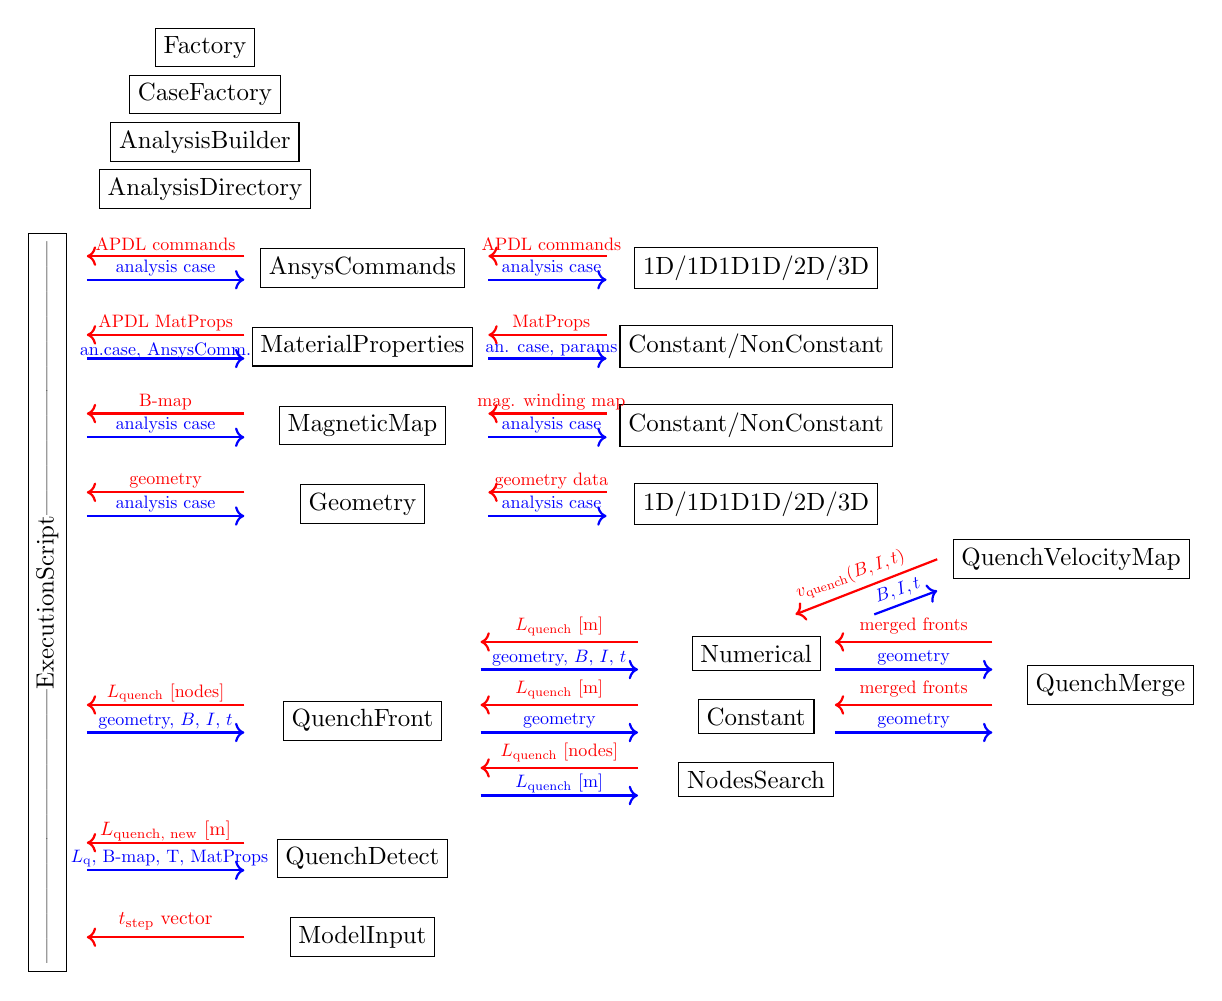
\begin{tikzpicture}[scale = 1]
\node[scale = 0.9, rotate=90] at (1,-4.25) [draw] {|||||||||||ExecutionScript|||||||||||};

\node[scale = 0.9] at (3,2.8) [draw] {Factory};
\node[scale = 0.9] at (3,2.2) [draw] {CaseFactory};
\node[scale = 0.9] at (3,1.6) [draw] {AnalysisBuilder};
\node[scale = 0.9] at (3,1) [draw] {AnalysisDirectory};

\node[scale = 0.9] at (5,0) [draw] {AnsysCommands};
\node[scale = 0.9] at (10,0) [draw] {1D/1D1D1D/2D/3D};
\draw [thick, red, ->] (3.5,0.15) -- (1.5,0.15);
\node[scale = 0.65, red] at (2.5,0.3) {APDL commands};
\draw [thick, blue, ->] (1.5,-0.15) -- (3.5,-0.15);
\node[scale = 0.65, blue] at (2.5,0) {analysis case};
\draw [thick, red, ->] (8.1,0.15) -- (6.6,0.15);
\node[scale = 0.65, red] at (7.4,0.3) {APDL commands};
\draw [thick, blue, ->] (6.6,-0.15) -- (8.1,-0.15);
\node[scale = 0.65, blue] at (7.4,0) {analysis case};

\node[scale = 0.9] at (5,-1) [draw] {MaterialProperties};
\node[scale = 0.9] at (10,-1) [draw] {Constant/NonConstant};
\draw [thick, red, ->] (3.5,-0.85) -- (1.5,-0.85);
\node[scale = 0.65, red] at (2.5,-0.7) {APDL MatProps};
\draw [thick, blue, ->] (1.5,-1.15) -- (3.5,-1.15);
\node[scale = 0.65, blue] at (2.5,-1.05) {an.case, AnsysComm.};
\draw [thick, red, ->] (8.1,-0.85) -- (6.6,-0.85);
\node[scale = 0.65, red] at (7.4,-0.7) {MatProps};
\draw [thick, blue, ->] (6.6,-1.15) -- (8.1,-1.15);
\node[scale = 0.65, blue] at (7.4,-1.05) {an. case, params};

\node[scale = 0.9] at (5,-2) [draw] {MagneticMap};
\node[scale = 0.9] at (10,-2) [draw] {Constant/NonConstant};
\draw [thick, red, ->] (3.5,-1.85) -- (1.5,-1.85);
\node[scale = 0.65, red] at (2.5,-1.7) {B-map};
\draw [thick, blue, ->] (1.5,-2.15) -- (3.5,-2.15);
\node[scale = 0.65, blue] at (2.5,-2) {analysis case};
\draw [thick, red, ->] (8.1,-1.85) -- (6.6,-1.85);
\node[scale = 0.65, red] at (7.4,-1.7) {mag. winding map};
\draw [thick, blue, ->] (6.6,-2.15) -- (8.1,-2.15);
\node[scale = 0.65, blue] at (7.4,-2) {analysis case};

\node[scale = 0.9] at (5,-3) [draw] {Geometry};
\node[scale = 0.9] at (10,-3) [draw] {1D/1D1D1D/2D/3D};
\draw [thick, red, ->] (3.5,-2.85) -- (1.5,-2.85);
\node[scale = 0.65, red] at (2.5,-2.7) {geometry};
\draw [thick, blue, ->] (1.5,-3.15) -- (3.5,-3.15);
\node[scale = 0.65, blue] at (2.5,-3) {analysis case};
\draw [thick, red, ->] (8.1,-2.85) -- (6.6,-2.85);
\node[scale = 0.65, red] at (7.4,-2.7) {geometry data};
\draw [thick, blue, ->] (6.6,-3.15) -- (8.1,-3.15);
\node[scale = 0.65, blue] at (7.4,-3) {analysis case};

\node[scale = 0.9] at (5,-5.75) [draw] {QuenchFront};
\draw [thick, red, ->] (3.5,-5.55) -- (1.5,-5.55);
\node[scale = 0.65, red] at (2.5,-5.4) {$L_\text{quench}~\text{[nodes]}$};
\draw [thick, blue, ->] (1.5,-5.9) -- (3.5,-5.9);
\node[scale = 0.65, blue] at (2.5,-5.75) {geometry, $B$, $I$, $t$};

\node[scale = 0.9] at (10,-4.9) [draw] {Numerical};
\draw [thick, red, ->] (8.5,-4.75) -- (6.5,-4.75);
\draw [thick, blue, ->] (6.5,-5.1) -- (8.5,-5.1);
\node[scale = 0.65, red] at (7.5,-4.55) {$L_\text{quench}~\text{[m]}$};
\node[scale = 0.65, blue] at (7.5,-4.95) {geometry, $B$, $I$, $t$};

\node[scale = 0.9] at (10,-5.7) [draw] {Constant};
\draw [thick, red, ->] (8.5,-5.55) -- (6.5,-5.55);
\draw [thick, blue, ->] (6.5,-5.9) -- (8.5,-5.9);
\node[scale = 0.65, red] at (7.5,-5.35) {$L_\text{quench}~\text{[m]}$};
\node[scale = 0.65, blue] at (7.5,-5.75) {geometry};

\node[scale = 0.9] at (10,-6.5) [draw] {NodesSearch};
\draw [thick, red, ->] (8.5,-6.35) -- (6.5,-6.35);
\draw [thick, blue, ->] (6.5,-6.7) -- (8.5,-6.7);
\node[scale = 0.65, red] at (7.5,-6.15) {$L_\text{quench}~\text{[nodes]}$};
\node[scale = 0.65, blue] at (7.5,-6.55) {$L_\text{quench}~\text{[m]}$};

\node[scale = 0.9] at (14.5,-5.3) [draw] {QuenchMerge};
\draw [thick, red, ->] (13,-4.75) -- (11,-4.75);
\draw [thick, blue, ->] (11,-5.1) -- (13,-5.1);
\node[scale = 0.65, red] at (12,-4.55) {merged fronts};
\node[scale = 0.65, blue] at (12,-4.95) {geometry};

\draw [thick, red, ->] (13,-5.55) -- (11,-5.55);
\draw [thick, blue, ->] (11,-5.9) -- (13,-5.9);
\node[scale = 0.65, red] at (12,-5.35) {merged fronts};
\node[scale = 0.65, blue] at (12,-5.75) {geometry};

\node[scale = 0.9] at (14,-3.7) [draw] {QuenchVelocityMap};
\draw [thick, red, ->] (12.3,-3.7) -- (10.5,-4.4);
\draw [thick, blue, ->] (11.5,-4.4) -- (12.3,-4.1);
\node[scale = 0.65, red, rotate=19] at (11.2,-3.9) {$v_\text{quench} (B,I,t)$};
\node[scale = 0.65, blue, rotate=19] at (11.8,-4.1) {$B,I,t$};

\node[scale = 0.9] at (5,-7.5) [draw] {QuenchDetect};
\draw [thick, red, ->] (3.5,-7.3) -- (1.5,-7.3);
\draw [thick, blue, ->] (1.5,-7.65) -- (3.5,-7.65);

\node[scale = 0.7, red] at (2.5,-7.15) {$L_\text{quench, new}$ [m]};
\node[scale = 0.65, blue] at (2.55,-7.5) {$L_\text{q}$, B-map, T, MatProps};

\node[scale = 0.9] at (5,-8.5) [draw] {ModelInput};
\draw [thick, red, ->] (3.5,-8.5) -- (1.5,-8.5);
\node[scale = 0.7, red] at (2.5,-8.3) {$t_\text{step}$ vector};
\end{tikzpicture}
\caption{Python script architecture}
\label{fig:python_script_architecture}
\end{figure}

Fig. \ref{fig:python_script_architecture} describes the Python code consisting of 4 different Classes and one executive script. The \textit{executive\_script} launches the simulation and executes pre-processing, solution as well as post-processing part of ANSYS simulation. It uses the Class \textit{ansys} to translate Python functions into APDL scripting language. The Class \textit{geometry} imports a meshed geometry and assigns the position in space for each node. Then, the class \textit{quench\_velocity} assigns new quench front position at each time step depending on a current quench velocity. Since the Class \textit{quench\_velocity} operates in meters, it requires a separate class \textit{node\_search} which maps a node number for the calculated quench length as described in Section \ref{subsection:node_searching_algorithm}.\\

At this stage, the class \textit{quench\_velocity} assumes that the quench velocity is constant. In further steps, the quench velocity will be estimated in two-way coupling manner as described in Section \ref{subsection:quench_velocity_algorithm}. In order to reach this step, a new Class called \textit{quench\_detection} will be created. It will initialize the new quench front as soon as the critical temperature is achieved outside of the quenched zone of the coil (turn to turn heat propagation).

% SKEW QUADRUPOLE ANALYSIS - QUENCH DETECTION
\clearpage
\section{Skew Quadrupole Quench Detection Analysis}
\label{section:skew_quadrupole_quench_detection_analysis}

This chapter describes the thermal quench analysis of a skew quadrupole developed by LASA laboratories of INFN-Milano. The skew quadrupole belongs to the group of high-order corrector magnets designed for the upgrade of High-Luminosity LHC. Their design assumes using no quench protection devices such as quench heaters or CLIQ except for crowbars \footnote{Describe what crowbars are...}. Therefore, when any of these magnet quenches, the discharge of energy stored in their magnetic field occurs merely by their own rise in resistivity. i.e. they are self-protected.

Quench velocity approach presented in chapter \ref{section:quench_velocity_modelling} is used to analyze the magnet as a 3-dimensional thermal domain. It is verified by comparing the available measurements of a quenched skew quadrupole with the simulation results conducted in ANSYS. One has to remember that the skew quadrupole is the only high-order corrector which has quench protection system installed, i.e. it is not self-protected. However, it has been used for illustration purposes because of its available quench measurements when quench heaters were not used. 

\subsection{Geometry}

Most of the data about the skew quadrupole was presented in Section~\ref{section: 1d_quench_propagation_geometry}. Unlike in 1D analyses presented in previous chapters, when a 3D thermal simulation of a magnet is considered, it is important to specify its winding scheme because the windings interact with each other thermally across the insulation layer. Fig.~\ref{fig:skew_quad_transversal_cross_section} shows the transversal cross-section of one coil of the skew quadrupole. The windings are enclosed within an area of 24.5x27.3~mm. Moreover, each coil is covered with a 1 mm-thick ground insulation layer apart from the insulation between each winding described in Section~\ref{section: 1d_quench_propagation_geometry}. The ground insulation on the internal side of the coil is thinner and equal to 0.15~mm.

\begin{figure}[H]
    \centering
    \begin{tikzpicture}
    \pgftext{\includegraphics[width=\linewidth]{sections/skew_quad_q_det/figures/skew_quad_design/skew_quad_transversal_cross_section.png}} at (0,0);
    \node[red] at (6.0,2.1) {layers};
    \node[red, rotate=90] at (4.3,0) {turns};
    \draw[red, very thick, dashed] (0.47,-0.95) -- (0.47,2.4); 
    \node[red, scale=0.8] at (1.9,2.1) {coil symmetry};
    \draw[black, very thick, ->] (-4.3,2.1) -- (-4.8,1.8); 
    \node[black, scale=0.8] at (-3.0,2.1) {ground insulation};
    \end{tikzpicture}
    \caption{The transversal cross-section of one coil of a skew quadrupole~\cite{marco_prioli_mails}.}
    \label{fig:skew_quad_transversal_cross_section}
\end{figure}

As shown in Fig.~\ref{fig:winding_arrangement_cross_section}, each coil has 29 turns in each of its 26 layers. In total, the number of windings per coil is 754~\cite{marco_prioli_mails, hl_lhc_tech_design_report_v01}.

\begin{figure}[H]
\centering
    \begin{tikzpicture}
        \begin{axis}[
          width=0.5\linewidth, 
          height=0.5\linewidth,
          xtick={0.0, 24.46},
          ytick={0.0, 27.30},
          xlabel={$x,~\text{mm}~\text{(layers direction)}$},
          ylabel={$y,~\text{mm}~\text{(turns direction)}$},
          xmajorgrids=true,
          ymajorgrids=true,
          xmin=-5.0,
          xmax=29.47,
          ymin=-5.0,
          ymax=32.29,
          ]
          \addplot[blue, only marks, mark size=1pt] table[x=x,y=y,col sep=comma] {sections/skew_quad_q_det/figures/skew_quad_design/winding_location_cross_section.csv};
        \end{axis}
        \draw[scale=0.172, red, very thick, dashed] (2.5,2) -- (2.5,33.0); 
        \node[red, scale=0.8] at (1.9,5.6) {coil symmetry};
        
    \end{tikzpicture}
    \caption{Location of the windings in the cross-section of a half-coil.}
    \label{fig:winding_arrangement_cross_section}
\end{figure}

The winding scheme is shown in Fig.~\ref{fig:winding_scheme_cross_section}. The winding~1 is placed at the bottom left of the 2D cross-section. The last winding number 754 is placed further in the \textit{x}-direction. The \nth{2} half of the coil is a~mirror reflection of the presented winding scheme.

\begin{figure}[H]
\centering
    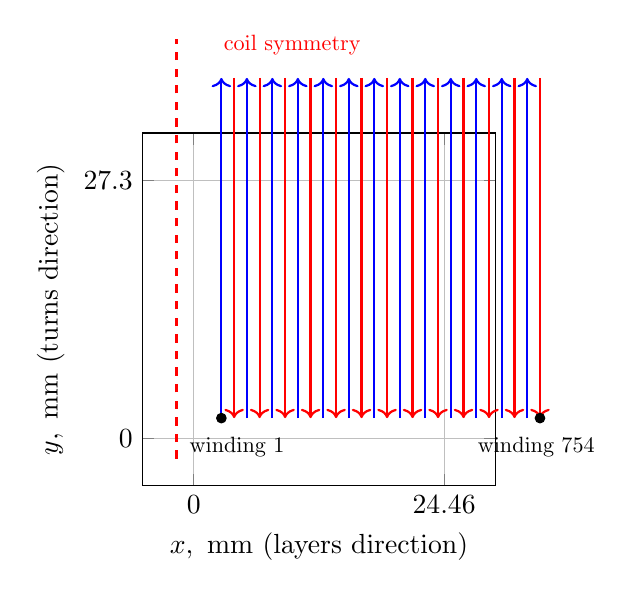
\begin{tikzpicture}
        \begin{axis}[
          width=0.5\linewidth, 
          height=0.5\linewidth,
          xtick={0.0, 24.46},
          ytick={0.0, 27.30},
          xlabel={$x,~\text{mm}~\text{(layers direction)}$},
          ylabel={$y,~\text{mm}~\text{(turns direction)}$},
          xmajorgrids=true,
          ymajorgrids=true,
          xmin=-5.0,
          xmax=29.47,
          ymin=-5.0,
          ymax=32.29,
          ]
        \end{axis}
        \foreach \t in {0.471, 2.353,...,24}
            \draw[scale=0.172, blue, thick, ->] (\t+5.35,5.0) -- (\t+5.35,26.819+3.3); 
        \foreach \t in {1.412, 3.294,...,25}
            \draw[scale=0.172, red, thick, ->] (\t+5.35,26.819+3.3) -- (\t+5.35,5.0);
        \draw[scale=0.172, red, very thick, dashed] (2.5,2) -- (2.5,33.0); 
        \node[red, scale=0.8] at (1.9,5.6) {coil symmetry};
        \filldraw[scale=0.172, black] (0.471+5.35,5.0) circle (10pt);
        \node[black, scale=0.8] at (1.2,0.5) {winding 1};
        \filldraw[scale=0.172, black] (23.996+5.35,5.0) circle (10pt);
        \node[black, scale=0.8] at (5.0,0.5) {winding 754};
        
    \end{tikzpicture}
    \caption{Winding scheme of a single coil of the skew quadrupole.}
    \label{fig:winding_scheme_cross_section}
\end{figure}

The general parameters of the skew quadrupole are summarised in Table~\ref{table:skew_quad_params_table}. In the given magnet, there is only one aperture in which a particle beam travels through. Four coils of the magnet are connected in series and powered by a single power converter. It is interesting to mention that the coil length of only one coil is more than 800~m which is a very large number for thermal quench simulations, as mentioned in Section~\ref{section: 1D_quench_propagation_conclusions}. The operating current of the skew quadrupole is $I=182~\text{A}$.

\begin{table}[H]
    \caption{Geometrical parameters for skew quadrupole \cite{marco_prioli_mails, hl_lhc_tech_design_report_v01}} 
    \vspace{-1.em} 
    \fontsize{10}{10}
    \selectfont 
    \renewcommand{\arraystretch}{1.5}
    \begin{center}
    \begin{tabular}{ ccc }  
    \hline
    parameter & value & unit \\
    \hline
    number of apertures & 1 & [-] \\
    number of circuits & 1 & [-] \\
    aperture size & 150 & [mm]\\
    coil length & 841 & [m] \\
    operating current & 182 & [A] \\
    \hline 
    \end{tabular}
    \end{center}  
     \label{table:skew_quad_params_table} 
 \end{table}

\subsection{Assumptions for Geometry and Material Properties}

Each cable is a single Nb-Ti strand of 0.7 mm diameter with a copper stabilizer. As presented in Fig. \ref{fig:materials_cross_section}, the winding is covered with 0.007 mm thick S2-glass insulation (in red). Then, the winding is immersed in epoxy resin D10 (in blue). The superconducting cable is marked in yellow. Moreover, ground insulation is added on the external side of the coil \cite{hl_lhc_tech_design_report_v01}.

In the superconducting magnet design community, an assumption is often proposed to simulate the materials behaviour outside of the superconducting cable as a single domain characterized by the properties of G10 which is another material widely used in cryogenics. Such an assumption is made in this thesis. The characteristics of all material properties taken into consideration in the analysis are described in Appendix \ref{appendix_material_properties_description}.

\begin{figure}[H]
\centering

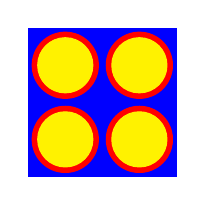
\begin{tikzpicture}[scale = 1]
\filldraw[blue] (-0.941/2,-0.941/2) rectangle (0.941/2,0.941/2);
\filldraw[red] (0,0) circle (0.7/2+0.07);
\filldraw[yellow] (0,0) circle (0.7/2);

\filldraw[blue] (-0.941/2,-0.941/2+0.941) rectangle (0.941/2,0.941/2+0.941);
\filldraw[red] (0,0+0.941) circle (0.7/2+0.07);
\filldraw[yellow] (0,0+0.941) circle (0.7/2);

\filldraw[blue] (-0.941/2+0.941,-0.941/2) rectangle (0.941/2+0.941,0.941/2);
\filldraw[red] (0+0.941,0) circle (0.7/2+0.07);
\filldraw[yellow] (0+0.941,0) circle (0.7/2);

\filldraw[blue] (-0.941/2+0.941,-0.941/2+0.941) rectangle (0.941/2+0.941,0.941/2+0.941);
\filldraw[red] (0+0.941,0+0.941) circle (0.7/2+0.07);
\filldraw[yellow] (0+0.941,0+0.941) circle (0.7/2);

\end{tikzpicture}
    \caption{Cross-section of four neighbouring windings}
    \label{fig:materials_cross_section}
\end{figure}

The stabilizer to superconductor ratio is specified in \cite{hl_lhc_tech_design_report_v01} and is calculated as follows:

\begin{equation}
    \left\{ \begin{array}{ll}
    \frac{f_\text{Cu}}{f_\text{Nb-Ti}} = \frac{A_\text{Cu}}{A_\text{Nb-Ti}} = 2.2\\ \\
    f_\text{Cu} + f_\text{Nb-Ti} = 1
    \end{array} \right.
\end{equation}

At temperatures above quench current flows through both superconductor and copper in parallel connection. What is actually quite surprising, resistivity of a superconductor above critical temperature is much higher that the one of copper. Therefore, it can be assumed that current flows through a stabilizer and only this part contributes to Joule heating. The same occurs with heat conductivity which is much lower for Nb-Ti at higher temperatures. In order to take these characteristics into account during numerical analysis, the winding area is reduced to area of copper. It leads to a formula of reduced diameter presented below.
\begin{equation}
    d_\text{strand, red} = \sqrt{\frac{A_\text{Cu}}{A_\text{strand}}}*d_\text{strand}
\end{equation}

Since the winding diameter in analysis is smaller than in reality, its equivalent heat capacity must take this correction into account which is shown in the equation below. The representative winding equivalent heat capacity is shown in Fig. \ref{fig:eq_wind_cp}.
\begin{equation}
    C_\text{p, equiv} = f_\text{Cu}*C_\text{p, Cu} + f_\text{NbTi}*C_\text{p, NbTi}
\end{equation}
 
\begin{figure}[h!]
    \centering
    \includegraphics[width=0.35\linewidth]{figures/material_properties/Eq_Cp_plot.png}
    \caption{Equivalent winding specific heat capacity temperature dependence for \textit{B}=3 T}
    \label{fig:eq_wind_cp}
\end{figure}

The geometrical data input are collected and specified altogether in Table \ref{table:skew_quad_params_table}.

\begin{table}[h!]
    \caption{Geometrical parameters for skew quadrupole \cite{hl_lhc_tech_design_report_v01, marco_prioli_mails}} 
    \vspace{-1.em} 
    \fontsize{10}{10}
    \selectfont 
    \renewcommand{\arraystretch}{1.5}
    \begin{center}
    \begin{tabular}{ ccc }  
    \hline
    Aperture & 150 & [mm]\\
    Coil length & 841 & [m] \\
    Number of apertures & 1 & \\
    Number of circuits & 1 & \\
    Strand diameter & 0.7 & [mm] \\
    $\text{A}_\text{Cu}/\text{A}_\text{Nb-Ti}$ \cite{marco_prioli_mails} & 2.2 & \\
    \hline 
    \end{tabular}
    \end{center}  
     \label{table:skew_quad_params_table} 
 \end{table}

Insulation dimensions:

\begin{equation}
    A_\text{ins} = a^2 - \frac{\pi d_\text{strand}^2}{4}
\end{equation}

\begin{equation}
    p_\text{avg} = \frac{4 a + \pi d_\text{strand}}{2} 
\end{equation}

\begin{equation}
    L_\text{ins} = \frac{A_\text{ins}}{p_\text{avg}}
\end{equation}

\begin{equation}
    A_\text{ins,cond} = \frac{\frac{1}{4} A_\text{ins} \cdot L_{winding}}{L_\text{ins}}
\end{equation}

\begin{figure}[H]
\centering
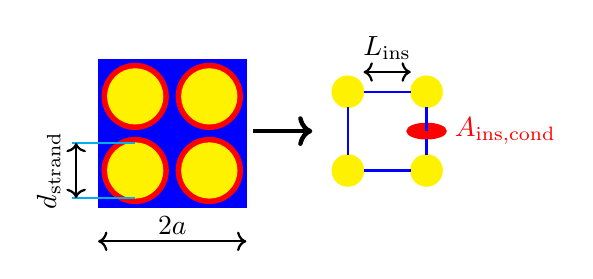
\begin{tikzpicture}[scale = 1]
\filldraw[blue] (-0.941/2,-0.941/2) rectangle (0.941/2,0.941/2);
\filldraw[red] (0,0) circle (0.7/2+0.07);
\filldraw[yellow] (0,0) circle (0.7/2);
\filldraw[blue] (-0.941/2,-0.941/2+0.941) rectangle (0.941/2,0.941/2+0.941);
\filldraw[red] (0,0+0.941) circle (0.7/2+0.07);
\filldraw[yellow] (0,0+0.941) circle (0.7/2);
\filldraw[blue] (-0.941/2+0.941,-0.941/2) rectangle (0.941/2+0.941,0.941/2);
\filldraw[red] (0+0.941,0) circle (0.7/2+0.07);
\filldraw[yellow] (0+0.941,0) circle (0.7/2);
\filldraw[blue] (-0.941/2+0.941,-0.941/2+0.941) rectangle (0.941/2+0.941,0.941/2+0.941);
\filldraw[red] (0+0.941,0+0.941) circle (0.7/2+0.07);
\filldraw[yellow] (0+0.941,0+0.941) circle (0.7/2);
\draw[thick, cyan] (-0.8,0.7/2) -- (0,0.7/2);
\draw[thick, cyan] (-0.8,-0.7/2) -- (0,-0.7/2);
\draw[black, thick, <->] (-0.75,0.7/2) -- (-0.75,-0.7/2);
\node[scale = 1, rotate=90] at (-1.1, 0) {$d_\text{strand}$};
\draw[thick,<->] (-0.941/2,-0.9) -- (0.941*1.5,-0.9);
\node[scale = 1] at (0.941*0.5, -0.7) {$2a$};
\draw[ultra thick,->, black] (1.5,0.5) -- (2.25,0.5);
\filldraw[yellow] (2.7,0) circle (0.2);
\filldraw[yellow] (3.7,0) circle (0.2);
\filldraw[yellow] (3.7,1) circle (0.2);
\filldraw[yellow] (2.7,1) circle (0.2);
\draw[thick, blue] (2.9,0) -- (3.5,0);
\draw[thick, blue] (2.9,1) -- (3.5,1);
\draw[thick, blue] (2.7,0.8) -- (2.7,0.2);
\filldraw[red] (3.7,0.5) ellipse (0.25cm and 0.1cm);
\draw[thick, blue] (3.7,0.8) -- (3.7,0.5);
\draw[thick, blue] (3.7,0.4) -- (3.7,0.2);
\draw[thick, black, <->] (2.9,1.25) -- (3.5,1.25);
\node[scale = 1] at (3.2, 1.55) {$L_\text{ins}$};
\node[scale = 1, red] at (4.7, 0.5) {$A_\text{ins,cond}$};
\end{tikzpicture}
\caption{Cross-sectional of 2D and 1D element}
\end{figure}


\subsection{Quench Measurements}

The quench measurements have been conducted for $I=86~\text{A}$ which is a lower value than the nominal operating current of the skew quadrupole ($I=182~\text{A}$). During the test, the quench has been initiated by discharging a capacitor in series with a 2x2 $\text{mm}^2$ heater attached to the external grounding insulation of the magnet. The voltage drop across the capacitor is presented in Fig. \ref{fig:resistor_voltage_discharge_curve}. By considering the discharge curve as the \nth{1} order, one can deduce the time constant and the resistance of the heater. The obtained data are presented in Table \ref{table:heater_characteristics}.

\begin{figure}[ht!]
    \centering
    \includegraphics[width=0.65\linewidth]{figures/skew_quad_bcs/voltage_discharge_curve.png}
    \caption{Voltage discharge across the capacitor (in blue) with it \nth{1} order discharge fit (in orange)}
    \label{fig:resistor_voltage_discharge_curve}
\end{figure}

\begin{table}[h!]
    \caption{Heater characteristics} 
    \vspace{-1.em} 
    \fontsize{10}{10}
    \selectfont 
    \renewcommand{\arraystretch}{1.5}
    \begin{center}
    \begin{tabular}{ ccc }  
    \hline
    capacitance & 14 & [mF] \\
    time constant & 3.5 & [ms] \\
    heater resistance & 0.25 & [$\Omega$] \\
    \hline 
    \end{tabular}
    \end{center}  
     \label{table:heater_characteristics} 
 \end{table}

Assuming an adiabatic hot spot (no helium effect), one can deduce total energy input to the magnet as well as power input as a function of time. Power function can be easily deduced from the equation below. The power curve is presented in Fig. \ref{fig:hot_spot_power_input_curve}. After $t=10~\text{ms}$, the value of power is negligible, i.e. the capacitor is fully discharged.
\begin{equation}
    P(t) = \frac{1}{\text{dt}} (\frac{1}{2} \text{C}V^2)
\end{equation}

\begin{figure}[ht!]
    \centering
    \includegraphics[width=0.45\linewidth]{figures/skew_quad_bcs/Polynomial_Power_Fit.png}
    \caption{Hot spot power input curve}
    \label{fig:hot_spot_power_input_curve}
\end{figure}

When the hot spot is applied, the individual windings start being normal conductive and, therefore resistive. The resistive voltage across the magnet increases, as presented in Fig. \ref{fig:res_volt_curve_quench_detection}. In skew quadrupole, the quench is detected if the magnet resistive voltage equal to at least $V=0.2~\text{V}$ last more than $t=20~\text{ms}$. At $t=0$, the power supply is cut off and the current starts decreasing.

\begin{figure}[ht!]
    \centering
    \includegraphics[width=0.6\linewidth]{figures/skew_quad_bcs/quench_det_v_curve.png}
    \caption{Resistive voltage rise until quench detection}
    \label{fig:res_volt_curve_quench_detection}
\end{figure}

\subsection{Magnetic Field Mapping}
Until the quench is detected, the current inside the magnet is constant and equal to $I=86~\text{A}$. Therefore, the magnetic field inside the magnet does not vary in time. The analysis of steady-state magnetic field in the middle of the magnet for this value of current was conducted at INFN-Milano in OPERA software \cite{samuele_mariotto_mails}. A 2D interpolation had to be conducted in order to fit the OPERA mesh with the windings' position. For each winding, it is assumed that it is subjected to the magnetic field from the centre of its cross-section estimated by the interpolation map presented in Fig. \ref{fig:Quad_Mag_contour1}.

\begin{figure}[ht!]
    \centering
    \includegraphics[width=0.49\linewidth]{figures/skew_quad_bcs/magnetic_field_mapping/Quadrupole_Magnetic_Colour_plot.png}
    \caption{Resultant magnetic field strength in the cross-section of skew quadrupole}
    \label{fig:Quad_Mag_contour1}
\end{figure}

\subsection{Initial Conditions...}

Thermal diffusivity is calculated as follows: 
\begin{equation}
    \alpha_{strand} = \frac{k_{Cu}}{\rho_{Cu} \cdot C_{p, equiv}}
\end{equation}

\begin{figure}
\centering
\begin{tikzpicture}
\begin{axis}[
  no markers,
  legend style={at={(1,0)},anchor=south east},
  grid=both, 
  grid style={dashed,gray!30},
  width=0.85\linewidth, 
  height = 6cm,
  xlabel={$T,~\text{K}$},
  ylabel={$\alpha,~\text{m}^2\text{s}^{-1}$},
  xlabel style={below right},
  ylabel style={above left},
%   minor xtick={5,10,...,25},
  xmin=1.0,
  ymin=0.0,
  xmax=25.0
  ]
  
  \addplot table[x=Time,y=diff_strand,col sep=comma] {figures/skew_quad_bcs/strand_th_diffusivity.csv}; 

\end{axis}
\end{tikzpicture}
\caption{Thermal diffusivity of the superconducting cable}
    \label{fig:strand_diffusivity_plot}
\end{figure}


\begin{figure}[H]
\centering
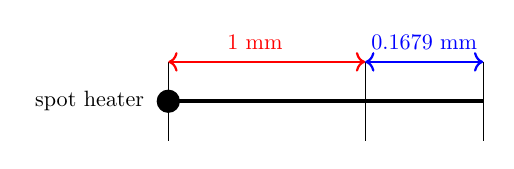
\begin{tikzpicture}[scale = 1]

\filldraw [black] (0,0) circle (4pt);
\draw [ultra thick] (0.0,0.0) -- (4.0,0);

\draw [thin] (2.5,-0.5) -- (2.5,0.5);
\draw [thin] (4.0,-0.5) -- (4.0,0.5);
\draw [thin] (0.0,-0.5) -- (0.0,0.5);

\draw [thick, <->, red] (0.0,0.5) -- (2.5,0.5);
\draw [thick, <->, blue] (2.5,0.5) -- (4.0,0.5);

\node[scale=0.8, color = black] at (-1.0,0.0) {spot heater};
\node[scale=0.8, color = red] at (1.1,0.75) {1 mm};
\node[scale=0.8, color = blue] at (3.25,0.75) {0.1679 mm};

\end{tikzpicture}
\caption{Schematic of 1D insulation modelling; simulation length as a sum of ground insulation (in red) and winding insulation (in blue) connected in series.}
\end{figure}


\clearpage

\subsection{Quench Velocity Mapping}

Quench velocity before quench detection has been estimated numerically. The magnetic field inside the magnet varies in the range of $B \in (0, 3)~\text{T}$. Therefore, 7 separate 1D analysis have been conducted in ANSYS to estimate quench velocity as a function of time and magnetic field.

\begin{figure}[ht!]
    \centering
    \includegraphics[width=0.6\linewidth]{figures/skew_quad_bcs/magnetic_field_mapping/Quench_Velocity_Map.png}
    \caption{Quench Velocity as a function of time and magnetic field strength}
    \label{fig:Q_v_map}
\end{figure}

\begin{figure}[H]
\centering
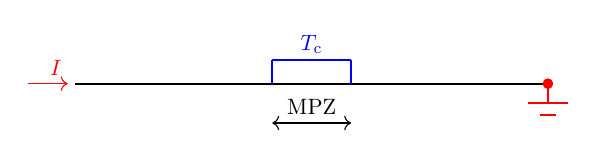
\begin{tikzpicture}[scale = 1]
\draw[thick, black] (-3,0) -- (3,0);
\filldraw[red] (3,0) circle (0.06);
\draw[thick, red] (3,0) -- (3,-0.25);
\draw[thick, red] (2.75,-0.25) -- (3.25,-0.25);
\draw[thick, red] (2.9,-0.4) -- (3.1,-0.4);
\draw[thin, red, ->] (-3.6,0) -- (-3.1,0);
\draw[thick, blue] (-0.5,0) -- (-0.5,0.3);
\draw[thick, blue] (-0.5,0.3) -- (0.5,0.3);
\draw[thick, blue] (0.5,0.3) -- (0.5,0);
\draw[thin, black, <->] (-0.5,-0.5) -- (0.5,-0.5);
\node[scale=0.8] at (0,-0.3) {MPZ};
\node[scale=0.8, blue] at (0,0.5) {$T_\text{c}$};
\node[scale=0.8, red] at (-3.25,0.2) {$I$};
\end{tikzpicture}
\caption{Simulation settings}
\label{fig:sim_settings_1}
\end{figure}

\begin{figure}[H]
\centering
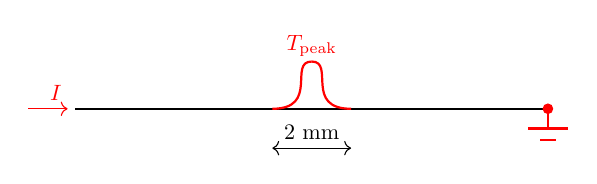
\begin{tikzpicture}[scale = 1]
\draw[thick, black] (-3,0) -- (3,0);
\filldraw[red] (3,0) circle (0.06);
\draw[thick, red] (3,0) -- (3,-0.25);
\draw[thick, red] (2.75,-0.25) -- (3.25,-0.25);
\draw[thick, red] (2.9,-0.4) -- (3.1,-0.4);
\draw[thin, red, ->] (-3.6,0) -- (-3.1,0);
\draw [thick, red] (-0.5,0) .. controls +(0:0.6cm) and +(180:0.3cm) .. (0,0.6);
\draw [thick, red] (0,0.6) .. controls +(0:0.3cm) and +(180:0.6cm) .. (0.5,0);
\draw[thin, black, <->] (-0.5,-0.5) -- (0.5,-0.5);
\node[scale=0.8] at (0,-0.3) {2 mm};
\node[scale=0.8, red] at (0,0.8) {$T_\text{peak}$};
\node[scale=0.8, red] at (-3.25,0.2) {$I$};
\end{tikzpicture}
\caption{Simulation settings}
\label{fig:sim_settings_2}
\end{figure}

\begin{figure}[H]
\centering
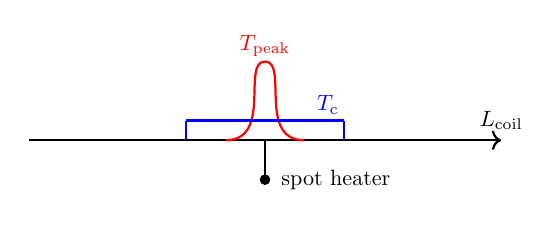
\begin{tikzpicture}[scale = 1]
\draw[thick, black, ->] (-3,0) -- (3,0);
\filldraw[black] (0,-0.5) circle (0.06);
\draw[thick, black] (0,0) -- (0,-0.5);
\draw [thick, red] (-0.5,0) .. controls +(0:0.6cm) and +(180:0.3cm) .. (0,1);
\draw [thick, red] (0,1) .. controls +(0:0.3cm) and +(180:0.6cm) .. (0.5,0);
\draw[thick, blue] (-1,0) -- (-1,0.25);
\draw[thick, blue] (-1,0.25) -- (1,0.25);
\draw[thick, blue] (1,0.25) -- (1,0);
\node[scale=0.8, black] at (0.9,-0.5) {spot heater};
\node[scale=0.8, black] at (3,0.25) {$L_\text{coil}$};
\node[scale=0.8, blue] at (0.8,0.45) {$T_\text{c}$};
\node[scale=0.8, red] at (0,1.2) {$T_\text{peak}$};
\end{tikzpicture}
\end{figure}

\begin{figure}[H]
\centering
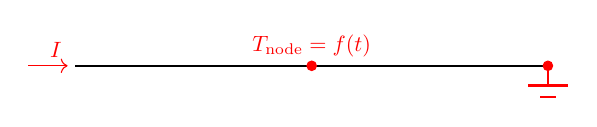
\begin{tikzpicture}[scale = 1]
\draw[thick, black] (-3,0) -- (3,0);
\filldraw[red] (3,0) circle (0.06);
\draw[thick, red] (3,0) -- (3,-0.25);
\draw[thick, red] (2.75,-0.25) -- (3.25,-0.25);
\filldraw[red] (0,0) circle (0.06);
\draw[thick, red] (2.9,-0.4) -- (3.1,-0.4);
\draw[thin, red, ->] (-3.6,0) -- (-3.1,0);
\node[scale=0.8, red] at (0,0.25) {$T_\text{node}= f(t)$};
\node[scale=0.8, red] at (-3.25,0.2) {$I$};
\end{tikzpicture}
\caption{Simulation settings}
\label{fig:sim_settings_3}
\end{figure}


% Analysis assumptions:
% No helium cooling
% Power input heats up the coil directly (no intermediate insulation layer) 
% Temperature in the windings’ cross-sectional area is uniform - 1D element
% Longitudinal heat transfer inside the insulation is negligible with respect to windings - 1D element


% Winding: 	link68, thermo-electric 1D elements for heat conduction + Joule heating
% Insulation: 	link33, thermal 1D elements for heat conduction



% Resistive voltage curve changes the slope during the analysis, - turn-to-turn propagation occurs in the model

% Turn-to-turn propagation occurs to slow compared to measurements-assumptions related to insulation elements are too conservative

% In measurements, quench spot is applied through insulation  direct power input in simulations ought to be modified

% Exact value of RRR of the measured magnet needs to be verified with INFN 


% Preparation of thermo-magneto-electric model to simulate current discharge

% Preparation of magnetic model in ANSYS to simulate magnetic field change during discharge (influence of iron yoke)
% Coupling of ANSYS quench velocity model with circuit in PSpice 
% Validation against measurements from INFN


\begin{figure}
\centering
\begin{tikzpicture}
\pgfplotsset{
    scale only axis,
    height=4cm,
    width=8cm,
    compat=1.3,
    scaled x ticks=base 10:0,
    xmin=0, xmax=9
}
\begin{axis}[
  axis y line*=left,
  ymin=0, ymax=20,
  xlabel={Time, s},
  ylabel={Resistive Voltage, V},
]
\addplot[smooth, red] table[x=Time,y=Resistive_Voltage,col sep=comma] {figures/skew_quad_bcs/current_voltage_discharge.csv}; 
\label{plot_resistive_voltage}
\end{axis}

\begin{axis}[
  axis y line*=right,
  axis x line=none,
  ymin=0, ymax=100,
  ylabel={Current, A}
]
\addplot[smooth, blue] table[x=Time,y=Current,col sep=comma] {figures/skew_quad_bcs/current_voltage_discharge.csv}; 
\label{current}
\addlegendentry{$I$}
\addlegendimage{/pgfplots/refstyle=plot_resistive_voltage}\addlegendentry{$V_\text{r}$}
\end{axis}
\end{tikzpicture}
\caption{Current and Resistive Voltage change during the discharge of skew quadrupole}
\label{fig:skew_quad_discharge}
\end{figure}


\begin{figure}
\centering
\begin{tikzpicture}
\pgfplotsset{
    scale only axis,
    height=4cm,
    width=8cm,
    compat=1.3,
    scaled x ticks=base 10:3,
    xmin=0, xmax=0.15
}
\begin{axis}[
  axis y line*=left,
  ymin=0, ymax=0.35,
  xlabel={Time, s},
  ylabel={Resistive Voltage, V},
]
\addplot[smooth, red] table[x=Time,y=Resistive_Voltage,col sep=comma] {figures/skew_quad_bcs/current_voltage_quench_detection.csv}; 
\label{plot_resistive_voltage}
\end{axis}

\begin{axis}[
  axis y line*=right,
  axis x line=none,
  ymin=0, ymax=100,
  ylabel={Current, A},
  legend pos=south east
]
\addplot[smooth, blue] table[x=Time,y=Current,col sep=comma] {figures/skew_quad_bcs/current_voltage_quench_detection.csv}; 
\label{current}
\addlegendentry{$I$}
\addlegendimage{/pgfplots/refstyle=plot_resistive_voltage}\addlegendentry{$V_\text{r}$}
\end{axis}
\end{tikzpicture}
\caption{Current and Resistive Voltage change during the discharge of skew quadrupole}
\label{fig:skew_quad_discharge}
\end{figure}

% APPENDICES
\clearpage
\begin{appendices}

\section{Material Properties}
\label{appendix_material_properties_description}

The material properties are based on an update of ROXIE database prepared at CERN \cite{material_properties_roxie}. Except for Nb-Ti specific heat capacity, NIST standards for cryogenic materials are used to describe them. Nb-Ti is defined by CUDI which is Arjan Verweij's software for Rutherford cable modelling~\cite{cudi_manual}.  

\subsection{Copper}
\label{appendix:cu_material_properties}

\subsubsection{Resistivity}
Copper resistivity depends on temperature and RRR:
\begin{equation}
    \rho_\text{N}(T, \text{RRR}) = \rho_\text{0}+\rho_\text{i}+\rho_\text{i0},
\end{equation}
\\
where:
\begin{equation}
    \rho_\text{0} = \frac{1.5553\cdot10^{-8}}{\text{RRR}}
\end{equation}

\begin{equation}
    \rho_\text{i} = \frac{\text{P}_\text{1}}{1+\text{P}_\text{1}  \text{P}_\text{3}  T^{\text{P}_\text{2} - \text{P}_\text{4}}  \exp{[-(\frac{\text{P}_\text{5}}{T}}^{\text{P}_\text{6}})]}
\end{equation}

\begin{equation}
    \rho_\text{i0} = \text{P}_\text{7} \frac{\rho_\text{i} \rho_\text{0}}{\rho_\text{i} + \rho_\text{0}}
\end{equation}
\\
In order to apply the resistivity dependence on magnetic field strength, the following formula are applied with fit parameters presented in Table \ref{table:nist_resistivity_parameters}:
\begin{equation}
    \rho_\text{N}(T, B, \text{RRR}) = \rho_\text{N}(T, \text{RRR}) \cdot (1 + 10^{a(x)}),  
\end{equation}
\\
where:
\begin{equation}
    a(x) = \sum_{n=0}^{N} a_\text{n}(\log_\text{10}x)^{n}
\end{equation}

\begin{equation}
    x \approx \frac{1.553 \cdot 10^{-8}}{\rho_\text{N}(T, \text{RRR})} \cdot B
\end{equation}

\begin{table}[h!]
    \caption{Fit parameters for NIST copper electrical resistivity} 
    \vspace{-1.em} 
    \fontsize{10}{10}
    \selectfont 
    \renewcommand{\arraystretch}{1.5}
    \begin{center}
    \begin{tabular}{ ccccccc }  
    \hline
    $\text{P}_1$ & $\text{P}_2$ & $\text{P}_3$ & $\text{P}_4$ & $\text{P}_5$ & $\text{P}_6$ & $\text{P}_7$ \\
    \hline
    $1.171\cdot10^{-17}$ & 4.49 & $3.841\cdot10^{10}$ & 1.14 & 50 & 6.428 & 0.4531 \\
    \hline 
    \end{tabular}
    \\
    \begin{tabular}{ ccccc }  
    $\text{a}_0$ & $\text{a}_1$ & $\text{a}_2$ & $\text{a}_3$ & $\text{a}_4$ \\
    \hline
    -2.662 & 0.3168 & 0.6229 & -0.1839 & 0.001827 \\
    \hline
    \end{tabular}
    \end{center}  
     \label{table:nist_resistivity_parameters} 
 \end{table}

Fig. \ref{fig:cu_resistivity_plot} shows copper resistivity for low and high value of RRR. In general, it rises with temperature, decrease of RRR and increase of magnetic field strength.

\begin{figure}
\centering
\begin{tikzpicture}
\begin{axis}[
  no markers,
  legend style={at={(1,0)},anchor=south east},
  grid style={dashed,gray!30},
  width=0.85\linewidth, 
  height = 6cm,
  xlabel={$t$},
  ylabel={$\rho_{Cu}$},
  xlabel style={below right},
  ylabel style={above left},
  xmin=0.0,
  ymin=0.0,
  xmax=100.0
  ]
  
  \addplot table[x=Time,y=B_0_0_RRR_100,col sep=comma] {figures/material_properties/Cu_Rho_B_Depenedence.csv}; 
  \addplot table[x=Time,y=B_3_0_RRR_100,col sep=comma] {figures/material_properties/Cu_Rho_B_Depenedence.csv}; 
  \addplot table[x=Time,y=B_0_0_RRR_200,col sep=comma] {figures/material_properties/Cu_Rho_B_Depenedence.csv}; 
  \addplot table[x=Time,y=B_3_0_RRR_200,col sep=comma] {figures/material_properties/Cu_Rho_B_Depenedence.csv}; 
  
  \legend{$B(\text{RRR}=100)=0~\text{T}$,
  $B(\text{RRR}=100)=3~\text{T}$,
  $B(\text{RRR}=200)=0~\text{T}$,
  $B(\text{RRR}=200)=3~\text{T}$}

\end{axis}
\end{tikzpicture}
\caption{Copper resistivity temperature dependence for varying magnetic field and RRR}
    \label{fig:cu_resistivity_plot}
\end{figure}

%  thermal conductivity
\subsubsection{Thermal Conductivity}
Copper thermal conductivity depends on temperature and RRR:
\begin{equation}
    k_\text{N}(T, \text{RRR}) = \frac{1}{\text{W}_\text{0} + \text{W}_\text{i} + \text{W}_\text{i0}}, 
\end{equation}
\\ 
where:
\begin{equation}
    \text{W}_\text{0} = \frac{\beta}{T}
\end{equation}

\begin{equation}
    \text{W}_\text{i} = \frac{\text{P}_\text{1} T^{\text{P}_\text{2}}}{1+\text{P}_\text{1}  \text{P}_\text{3}  T^{\text{P}_\text{2} + \text{P}_\text{4}}  \exp{[-(\frac{\text{P}_\text{5}}{T}}^{\text{P}_\text{6}})]}
\end{equation}

\begin{equation}
    \text{W}_\text{i0} = \text{P}_\text{7} \frac{\text{W}_\text{i} \text{W}_\text{0}}{\text{W}_\text{i} + \text{W}_\text{0}}
\end{equation}
\\
with fit parameters presented in Table \ref{table:nist_cu_k_parameters}.

\begin{table}[h!]
    \caption{Fit parameters for NIST copper thermal conductivity} 
    \vspace{-1.em} 
    \fontsize{10}{10}
    \selectfont 
    \renewcommand{\arraystretch}{1.5}
    \begin{center}
    \begin{tabular}{ cc }  
    $\beta$ & $\beta_\text{r}$ \\
    \hline
    $0.634/\text{RRR}$ & $\beta/0.0003$ \\
    \hline
    \end{tabular}
    
    \begin{tabular}{ ccccccc }  
    $\text{P}_1$ & $\text{P}_2$ & $\text{P}_3$ & $\text{P}_4$ & $\text{P}_5$ & $\text{P}_6$ & $\text{P}_7$ \\
    \hline
    $1.754\cdot10^{-8}$ & 2.763 & 1102 & -0.165 & 70 & 1.756 & $0.838/\beta_\text{r}^{0.1661}$ \\
    \hline 
    \end{tabular}
    \end{center}  
     \label{table:nist_cu_k_parameters} 
 \end{table}
 
 In order to include the magnetic induction dependence in the function of thermal conductivity, one can apply: 
\begin{equation}
    k_\text{N}(T, B, \text{RRR}) = \frac{\rho\text{N}(T, B=0, \text{RRR})}{\rho\text{N}(T, B=0, \text{RRR})} \cdot k_\text{N}(T, \text{RRR})
\end{equation}

As presented in Fig. \ref{fig:cu_k_plot}, thermal conductivity decreases with increase of magnetic field strength and when a cable is characterised by lower RRR. One can also notice that the peak value of thermal conductivity occurs at lower temperatures when RRR is high. 
 
\begin{figure}[h!]
    \centering
    \includegraphics[width=0.49\linewidth]{figures/material_properties/Cu_k_B_Depenedence_plot_rrr_50.png}
    \includegraphics[width=0.49\linewidth]{figures/material_properties/Cu_k_B_Depenedence_plot_rrr_150.png}
    \caption{Copper thermal conductivity temperature dependence for three values of magnetic field for RRR = 50 (left) and RRR = 150 (right) }
    \label{fig:cu_k_plot}
\end{figure}

% mass density 
\subsubsection{Mass Density}
The mass density of copper is assumed to be constant and equal to $\rho = 8960~\text{kg/m}^{3}$.

% specific heat capacity 
\subsubsection{Specific Heat Capacity}
Copper specific heat capacity is approximated with the NIST polynomial interpolation. The fit with parameters described in Table \ref{table:nist_cu_cp_parameters}, is valid in the range between 4 and 300 K. It is assumed that the fit is valid throughout the entire analysis of quench.

\begin{equation}
    x(T) = 10^{\sum_{n=0}^{N} a_\text{n}(\log_\text{10}T)^{n}},
\end{equation}
\\
where $N$ refers to the order of polynomial.

\begin{table}[h!]
    \caption{Fit parameters for NIST copper specific heat capacity} 
    \vspace{-1.em} 
    \fontsize{10}{10}
    \selectfont 
    \renewcommand{\arraystretch}{1.5}
    \begin{center}
    \begin{tabular}{ cccccccc }  
    $\text{a}_0$ & $\text{a}_1$ & $\text{a}_2$ & $\text{a}_3$ & $\text{a}_4$ & $\text{a}_5$ & $\text{a}_6$ & $\text{a}_7$ \\
    \hline
    -1.91844 & -0.15973 & 8.61013 & -18.996 & 21.9661 & -12.7328 & 3.54322 & -0.3797 \\
    \hline 
    \end{tabular}
    \end{center}  
     \label{table:nist_cu_cp_parameters} 
 \end{table}

\begin{figure}[h!]
    \centering
    \includegraphics[width=0.49\linewidth]{figures/material_properties/Cu_Cp_plot.png}
    \caption{Copper specific heat capacity temperature dependence}
    \label{fig:cu_cp_plot}
\end{figure}
\newpage

% \subsection{Niobium Titanium}
% \label{appendix:nbti_material_properties}
% 
% NbTi mass density 
\subsubsection{Mass Density}
The mass density is assumed to be constant and equal to $\rho = 6000~\text{kg/m}^{3}$.

% NbTi specific heat capacity
\subsubsection{Specific Heat Capacity}
Volumetric heat capacity of Nb-Ti is estimated by means of a piece-wise polynomial function which takes into account a linear magnetic dependence below the critical temperature $T_\text{c}$. In order to obtain specific heat capacity in [$\frac{\text{J}}{\text{kg} \cdot \text{K}}$], the function is divided by a constant mass density. The fit parameters are presented in Table \ref{table:nbti_parameters}.

\begin{equation}
    \left\{ \begin{array}{ll}
    Cp_\text{ NbTi}(T, T_\text{c}) = \frac{\text{a}_0 + \text{a}_1\cdot T^{1} + \text{a}_2\cdot T^{2} + \text{a}_3\cdot T^{3}+ \text{a}_4\cdot T^{4}} {\rho_{Nb-Ti}} \\ \\
    T_\text{c}(B) = T_\text{c0}\cdot(1-\frac{B}{B_\text{c20}})^{0.59}
    \end{array} \right.
\end{equation}

\begin{table}[h!]
    \caption{Polynomial parameters} 
    \vspace{-1.em} 
    \fontsize{10}{10}
    \selectfont 
    \renewcommand{\arraystretch}{1.5}
    \begin{center}
    \begin{tabular}{ lccccc }  
    \hline
    & $\text{a}_0$ & $\text{a}_1$ & $\text{a}_2$ & $\text{a}_3$ & $\text{a}_4$ \\
    \hline
    $T \in (0, T_\text{c})$~K & 0 & $64 \cdot B$ & 0 & 49.1 & 0 \\        
    $T \in [T_\text{c}, 28.358)$~K & 0 & 928 & 0 & 16.24 & 0 \\        
    $T \in [28.358, 50.99)$~K & 41383 & -7846.1 & 553.71 & 11.9838 & -0.2177 \\        
    $T \in [50.99, 165.8)$~K & $-1.53\cdot10^{6}$ & 83022 & -716.3 & 2.976 & -0.00482 \\ 
    $T \in [165.8, 496.54)$~K & $1.24\cdot10^{6}$ & 13706 & -51.66 & 0.09296 & $-6.29\cdot10^{-5}$ \\        
    $T \in [496.54, 1000)$~K & $2.45\cdot10^{6}$ & 955.5 & -0.257 & 0 & 0 \\       
    \hline
     \end{tabular} 
    \end{center}  
     \label{table:nbti_parameters} 
 \end{table}
 
 \begin{figure}[h!]
    \centering
    \includegraphics[width=0.49\linewidth]{figures/material_properties/NbTi_Cp_B_Depenedence_plot.png}
    \caption{Nb-Ti specific heat capacity temperature dependence for two values of magnetic field}
    \label{fig:nbti_cp_plot}
\end{figure}
\newpage


% \subsection{G10 Material Properties}
% \label{appendix:g10_material_properties}
% 
% thermal conductivity
\subsubsection{Thermal Conductivity}
G10 is an epoxy-impregnated fiberglass, thermally anisotropic. It means that its thermal conductivity along the fibers is higher than across them. In order to simplify computation in the scope of this thesis, the material is assumed to be isotropic. A conservative assumption is made which states that thermal conductivity of G10 in all directions is equal to the one normal to the direction of the fibers.
G10 thermal conductivity as well as specific heat capacity is approximated with the NIST polynomial interpolation:
\begin{equation}
    x(T) = 10^{\sum_{n=0}^{N} a_\text{n}(\log_\text{10}T)^{n}},
\end{equation}
\\
where $N$ refers to the order of polynomial and $x(T)$ is the considered material property. Fig. \ref{fig:g10_k_plot} presents G10 heat conductivity based on polynomial fit parameters depicted in Table \ref{table:nist_g10_k_parameters}.

\begin{table}[h!]
    \caption{Fit parameters for NIST G10 thermal conductivity} 
    \vspace{-1.em} 
    \fontsize{10}{10}
    \selectfont 
    \renewcommand{\arraystretch}{1.5}
    \begin{center}
    \begin{tabular}{ ccccccccc }  
    $\text{a}_0$ & $\text{a}_1$ & $\text{a}_2$ & $\text{a}_3$ & $\text{a}_4$ & $\text{a}_5$ & $\text{a}_6$ & $\text{a}_7$ & $\text{a}_8$ \\
    \hline
    -4.1236 & 13.788 & -26.068 & 26.272 & -14.663 & 4.4954 & -0.6905 & 0.0397 & 0 \\
    \hline 
    \end{tabular}
    \end{center}  
     \label{table:nist_g10_k_parameters} 
 \end{table}
 
  \begin{figure}[h!]
    \centering
    \includegraphics[width=0.49\linewidth]{figures/material_properties/G10_k_plot.png}
    \caption{G10 heat conductivity temperature dependence}
    \label{fig:g10_k_plot}
\end{figure}
 
% mass density
 \subsubsection{Mass Density}
 The mass density is assumed to be constant and equal to $\rho = 1948~\text{kg/m}^{3}$ according to NIST standards.

% specific heat capacity
\subsubsection{Specific Heat Capacity}
Fig. \ref{fig:g10_cp_plot} presents G10 specific heat capacity function based on polynomial fit parameters depicted in Table \ref{table:nist_g10_cp_parameters}.

\begin{table}[h!]
    \caption{Fit parameters for NIST G10 specific heat capacity} 
    \vspace{-1.em} 
    \fontsize{10}{10}
    \selectfont 
    \renewcommand{\arraystretch}{1.5}
    \begin{center}
    \begin{tabular}{ cccccccc }  
    $\text{a}_0$ & $\text{a}_1$ & $\text{a}_2$ & $\text{a}_3$ & $\text{a}_4$ & $\text{a}_5$ & $\text{a}_6$ & $\text{a}_7$ \\
    \hline
    -2.4083 & 7.6006 & -8.2982 & 7.3301 & -4.2386 & 1.4294 & -0.24396 & 0.015236 \\
    \hline 
    \end{tabular}
    \end{center}  
     \label{table:nist_g10_cp_parameters} 
 \end{table}

 \begin{figure}[h!]
    \centering
    \includegraphics[width=0.49\linewidth]{figures/material_properties/G10_Cp_plot.png}
    \caption{G10 specific heat capacity temperature dependence}
    \label{fig:g10_cp_plot}
\end{figure}

\section{Compilation of ANSYS with Python Environment}
\label{appendix:python_ansys_compilation}

The representative code for Python compilation with ANSYS environment is presented in Table~\ref{table:ansys_python_compilation}.

\begin{table}[h!]
    \caption{Compilation of Python with ANSYS environment} 
    \vspace{-1em} 
    \fontsize{10}{10}
    \selectfont 
    \renewcommand{\arraystretch}{1}
    \begin{center}
    \begin{tabular}{ ll }  
    \hline  
        from ansys\_corba import CORBA & - imports ANSYS library \\
        os.chdir(directory) & - sets analysis directory\\
        with open('aaS\_MapdlID.txt', 'r') as f: \\ aasMapdlKey = f.read() & - opens APDL analysis \\
        mapdl = CORBA.ORB\_init().string\_to\_object(aasMapdlKey) & - creates mapdl object \\
    \hline
        mapdl.executeCommandToString("/prep7") & - exemplary command \\
     \end{tabular} 
    \end{center}  
     \label{table:ansys_python_compilation} 
 \end{table}
\newpage

% \section{Mapping Algorithm Python Script}
% \section{Quench Velocity Algorithm Python Script}
% \section{Nodes Search Algorithm Python Script}

\end{appendices}

\clearpage
\bibliographystyle{IEEEtran}
\bibliography{IEEEabrv,./bib/article}

\end{document}
